% ======================================================================
%  BÁO CÁO ĐỒ ÁN MTH055 — KHAI THÁC DỮ LIỆU LỚN — NHÓM 19
%  Biên dịch: pdfLaTeX
%     pdflatex main  ->  bibtex main  ->  pdflatex main  ->  pdflatex main
% ======================================================================
\documentclass[12pt,a4paper,oneside]{extreport}

% ------------------------- Tiếng Việt ---------------------------------
\usepackage[utf8]{vietnam}   % Bật Tiếng Việt: Chương, Hình, Bảng, Mục lục, Tài liệu tham khảo...

% ------------------------- Trình bày trang ----------------------------
% Lề theo yêu cầu đồ án MTH055: trên/dưới 2.5cm, trái 3cm (gáy), phải 2.5cm.
\usepackage[top=2.5cm, bottom=2.5cm, left=3.0cm, right=2.5cm]{geometry}
\usepackage{setspace}
\onehalfspacing                 % Giãn dòng 1.5
\usepackage{indentfirst}        % Thụt đầu dòng cho cả đoạn đầu tiên của mỗi mục
\setlength{\parindent}{1cm}
% Cho phép TeX co giãn thêm ở bước cuối để tránh chữ tràn ra ngoài lề, đặc biệt
% với các tên định danh dài ở dạng \texttt (vd: santander_satisfaction).
\setlength{\emergencystretch}{3em}
\setcounter{secnumdepth}{3}
\setcounter{tocdepth}{3}

% ------------------------- Toán học & môi trường định lý ----------------
\usepackage{amsmath,amssymb,amsthm,amsfonts,mathtools}
\theoremstyle{definition}
\newtheorem{dinhnghia}{Định nghĩa}[chapter]
\newtheorem{vidu}{Ví dụ}[chapter]
\newtheorem{nhanxet}{Nhận xét}[chapter]
\theoremstyle{plain}
\newtheorem{dinhly}{Định lý}[chapter]
\newtheorem{menhde}{Mệnh đề}[chapter]
\newtheorem{bode}{Bổ đề}[chapter]

% ------------------------- Hình & bảng --------------------------------
\usepackage{graphicx}
\graphicspath{{image/}}
\usepackage{float}
\usepackage{booktabs,tabularx,array,multirow,makecell,longtable}
\usepackage{caption,subcaption}
\captionsetup{font=small,labelfont=bf}

% ------------------------- Thuật toán ---------------------------------
\usepackage{algorithm}
\usepackage{algpseudocode}
\floatname{algorithm}{Thuật toán}
\renewcommand{\listalgorithmname}{Danh mục thuật toán}
\algrenewcommand\algorithmicrequire{\textbf{Đầu vào:}}
\algrenewcommand\algorithmicensure{\textbf{Đầu ra:}}
\algrenewcommand\algorithmicreturn{\textbf{trả về}}

% ------------------------- Mã nguồn -----------------------------------
\usepackage{listings}
\lstset{basicstyle=\ttfamily\footnotesize, breaklines=true, frame=single,
        columns=fullflexible, showstringspaces=false}

% ------------------------- Hình vẽ TikZ -------------------------------
\usepackage{pgfplots}
\pgfplotsset{compat=1.17}
\usepackage{tikz}
% Hình 3.1 chỉ dùng toạ độ tuyệt đối nên không phụ thuộc thư viện nào; các thư
% viện dưới đây nạp sẵn để phòng khi chỉnh sửa hình theo định vị tương đối.
\usetikzlibrary{positioning, shapes.geometric, arrows.meta}

% ------------------------- Màu / liên kết -----------------------------
\usepackage{xcolor}
\usepackage{url}
\usepackage[hidelinks]{hyperref}

% ------------------------- Định dạng tiêu đề chương -------------------
\usepackage{titlesec}
\titleformat{\chapter}[display]
  {\normalfont\Large\bfseries\centering}
  {\MakeUppercase{\chaptertitlename}\ \thechapter}{8pt}{\Large\MakeUppercase}
\titlespacing*{\chapter}{0pt}{6pt}{24pt}

% ======================================================================
\begin{document}

% ============================ PHẦN ĐẦU ================================
\pagenumbering{roman}          % Đánh số i, ii, iii... cho phần đầu

% ===================== TRANG BÌA ======================================
\begin{titlepage}
\centering
{\large ĐẠI HỌC QUỐC GIA THÀNH PHỐ HỒ CHÍ MINH\par}
{\large TRƯỜNG ĐẠI HỌC KHOA HỌC TỰ NHIÊN\par}
{\large KHOA CÔNG NGHỆ THÔNG TIN\par}
\vspace{0.3cm}
\rule{0.5\linewidth}{0.4pt}\par

% (Tuỳ chọn) Chèn logo trường:
% \includegraphics[width=3cm]{image/logo.png}\par
\vspace{1.2cm}

{\large ĐỒ ÁN MÔN HỌC\par}
{\large \textbf{KHAI THÁC DỮ LIỆU LỚN} (MTH055)\par}
\vspace{1.8cm}

{\Large\bfseries ĐÁNH GIÁ VÀ SO SÁNH CÔNG BẰNG\\[0.3cm]
CÁC FRAMEWORK AUTOML TRÊN DỮ LIỆU THỰC\par}
% Gợi ý tiêu đề khác (tuỳ nhóm chốt lại): "Xây dựng hệ thống benchmark AutoML
% tái lập được theo giao thức AMLB". Chỉnh cho khớp hướng tiếp cận cuối cùng.
\vspace{1.8cm}

{\large \textbf{Nhóm 19}\par}
\vspace{0.4cm}
% Liệt kê thành viên: Họ tên -- MSHV. Thay bằng thông tin thật của nhóm.
\begin{tabular}{ll}
{[}Họ và tên thành viên 1{]} & {[}MSHV{]} \\
{[}Họ và tên thành viên 2{]} & {[}MSHV{]} \\
{[}Họ và tên thành viên 3{]} & {[}MSHV{]} \\
{[}Họ và tên thành viên 4{]} & {[}MSHV{]} \\
\end{tabular}
\vspace{1.5cm}

{\large \textbf{Giảng viên hướng dẫn:} [Học hàm, học vị, Họ tên GVHD]\par}
\vspace{0.3cm}
{\large \textbf{Học kỳ:} Học kỳ 2, năm học 2025--2026\par}
\vfill

{\large THÀNH PHỐ HỒ CHÍ MINH -- 2026\par}
\end{titlepage}

% ===================== LỜI CAM ĐOAN ===================================
\chapter*{Lời cam đoan}
\addcontentsline{toc}{chapter}{Lời cam đoan}

Chúng tôi xin cam đoan báo cáo đồ án môn học \textit{``Đánh giá và so sánh công
bằng các framework AutoML trên dữ liệu thực''} là công trình nghiên cứu của Nhóm
19 dưới sự hướng dẫn của [Học hàm, học vị, họ tên giảng viên hướng dẫn]. Các nội
dung, số liệu và kết quả trình bày trong báo cáo là trung thực; các kết quả thực
nghiệm được tạo ra từ mã nguồn do nhóm xây dựng và được lưu trữ đầy đủ trong kho
mã nguồn của đề tài. Những tài liệu, ý tưởng và kết quả của tác giả khác khi được
sử dụng đều được trích dẫn và ghi rõ nguồn trong phần Tài liệu tham khảo. Việc sử
dụng công cụ hỗ trợ (bao gồm công cụ trí tuệ nhân tạo) được ghi chú minh bạch
trong Phụ lục. Nếu phát hiện có bất kỳ sự gian lận nào, chúng tôi xin hoàn toàn
chịu trách nhiệm.

\vspace{1.5cm}
\hfill
\begin{minipage}{0.45\linewidth}
\centering
Thành phố Hồ Chí Minh, [ngày] tháng [tháng] năm [năm]\\[0.3cm]
\textit{Nhóm/Tác giả thực hiện}\\[2.5cm]
[Họ và tên]
\end{minipage}

% ===================== LỜI CẢM ƠN =====================================
\chapter*{Lời cảm ơn}
\addcontentsline{toc}{chapter}{Lời cảm ơn}

[Viết lời cảm ơn: gửi tới giảng viên hướng dẫn, quý thầy cô bộ môn/khoa, gia
đình và bạn bè đã hỗ trợ trong quá trình thực hiện đề tài. Nên viết ngắn gọn,
chân thành, đúng văn phong trang trọng.]

\vspace{1.0cm}
\hfill \textit{[Nhóm/Tác giả thực hiện]}

% ===================== TÓM TẮT ========================================
\chapter*{Tóm tắt}
\addcontentsline{toc}{chapter}{Tóm tắt}

Học máy tự động (\textit{Automated Machine Learning}, AutoML) giúp tự động hoá
quá trình lựa chọn thuật toán và tinh chỉnh siêu tham số, nhờ đó rút ngắn đáng
kể công sức xây dựng mô hình. Tuy nhiên, việc so sánh các thư viện AutoML trong
thực tế thường thiếu công bằng và khó tái lập: mỗi thư viện được chạy với ngân
sách thời gian, cách chia dữ liệu, độ đo và tài nguyên khác nhau, đồng thời các
lần chạy thất bại thường bị bỏ qua thay vì được ghi nhận. Điều này khiến kết quả
so sánh dễ gây hiểu nhầm và khó kiểm chứng.

Trong đồ án này, nhóm tái hiện và mở rộng phương pháp đánh giá công bằng theo
chuẩn \textit{AutoML Benchmark} (AMLB) của Gijsbers và cộng sự, áp dụng cùng một
giao thức thống nhất (cùng cách chia fold, cùng ngân sách thời gian, cùng độ đo
và cùng tài nguyên) cho mọi thư viện trên mỗi tập dữ liệu, đồng thời ghi nhận
đầy đủ các lần chạy thất bại. Nhóm xây dựng một hệ thống \textit{AutoML Bench
Console} cho phép nạp dữ liệu (tải lên tệp CSV, lấy từ OpenML hoặc nhập liên kết
Kaggle công khai), tích hợp thư viện AutoML dưới dạng ảnh Docker, chạy đánh giá
và trực quan hoá kết quả, với dữ liệu được lưu trữ trên PostgreSQL và MinIO.

Nhóm tiến hành thực nghiệm so sánh ba thư viện AutoML tiêu biểu là FLAML,
H2O~AutoML và AutoGluon trên các tập dữ liệu phân lớp và hồi quy, sử dụng các độ
đo AUC, log-loss và RMSE, và xếp hạng các thư viện theo thứ hạng trung bình. Kết
quả sơ bộ cho thấy [tóm tắt phát hiện chính sau khi hoàn tất lần chạy đầy đủ], và
làm rõ sự đánh đổi giữa chất lượng mô hình và chi phí thời gian/tài nguyên giữa
các thư viện.

\vspace{0.5cm}
\noindent\textbf{Từ khoá:} học máy tự động (AutoML), đánh giá công bằng
(benchmark), khả năng tái lập, FLAML, H2O AutoML, AutoGluon.


\addcontentsline{toc}{chapter}{Mục lục}
\tableofcontents

\clearpage
\addcontentsline{toc}{chapter}{\listfigurename}
\listoffigures

\clearpage
\addcontentsline{toc}{chapter}{\listtablename}
\listoftables

% ===================== DANH MỤC THUẬT NGỮ VÀ VIẾT TẮT =================
\clearpage
\chapter*{Danh mục thuật ngữ và viết tắt}
\addcontentsline{toc}{chapter}{Danh mục thuật ngữ và viết tắt}

\begin{center}
\begin{tabularx}{\linewidth}{@{}l l X@{}}
\toprule
\textbf{Viết tắt} & \textbf{Thuật ngữ đầy đủ} & \textbf{Nghĩa / diễn giải} \\
\midrule
AutoML & Automated Machine Learning & Học máy tự động \\
AMLB   & AutoML Benchmark & Chuẩn đánh giá AutoML của Gijsbers và cộng sự \\
CASH   & Combined Algorithm Selection and Hyperparameter optimization & Bài toán chọn thuật toán và tối ưu siêu tham số kết hợp \\
CV     & Cross-Validation & Kiểm chứng chéo (chia dữ liệu theo fold) \\
AUC    & Area Under the ROC Curve & Diện tích dưới đường cong ROC \\
RMSE   & Root Mean Squared Error & Căn bậc hai sai số bình phương trung bình \\
HPO    & Hyperparameter Optimization & Tối ưu siêu tham số \\
NAS    & Neural Architecture Search & Tìm kiếm kiến trúc mạng nơ-ron \\
OpenML & Open Machine Learning & Nền tảng chia sẻ dữ liệu và tác vụ học máy \\
UI     & User Interface & Giao diện người dùng \\
\bottomrule
\end{tabularx}
\end{center}

% Bổ sung/loại bớt cho khớp với thuật ngữ thực sự xuất hiện trong báo cáo.


% ============================ NỘI DUNG ===============================
\clearpage
\pagenumbering{arabic}         % Đánh số 1, 2, 3... cho phần nội dung

% ======================================================================
%  CHƯƠNG 1 — MỞ ĐẦU
%  Yêu cầu (mục 2.2, 2.6 của đề bài): bối cảnh & động lực; phát biểu bài toán
%  (Input/Output/Ràng buộc); mục tiêu & phạm vi; đóng góp; cấu trúc báo cáo.
%  Độ dài tham khảo: 5--10 trang.
% ======================================================================
\chapter{Mở đầu}
\label{ch:gioithieu}

\section{Bối cảnh và động lực nghiên cứu}
\label{sec:boicanh}
Sự phổ biến của học máy trong nhiều lĩnh vực đã kéo theo nhu cầu ngày càng lớn
về việc xây dựng mô hình một cách nhanh chóng và hiệu quả. Tuy nhiên, một quy
trình học máy điển hình đòi hỏi nhiều bước thủ công đòi hỏi chuyên môn cao: tiền
xử lý dữ liệu, trích chọn đặc trưng, lựa chọn thuật toán và tinh chỉnh siêu tham
số. Học máy tự động (\textit{Automated Machine Learning}, AutoML) ra đời nhằm tự
động hoá các bước này, giúp người dùng không chuyên vẫn có thể thu được mô hình
chất lượng với công sức tối thiểu~\cite{feurer2015autosklearn}.

Hiện nay có nhiều thư viện AutoML mã nguồn mở phổ biến như FLAML~\cite{wang2021flaml},
H2O~AutoML~\cite{ledell2020h2o} và AutoGluon~\cite{erickson2020autogluon}, mỗi thư
viện dựa trên một triết lý thiết kế khác nhau. Điều này đặt ra một câu hỏi thực
tiễn quan trọng: \textit{với một bài toán và một ngân sách tài nguyên cho trước,
nên lựa chọn thư viện AutoML nào?} Trả lời câu hỏi này đòi hỏi một quá trình đánh
giá so sánh khách quan.

Trên thực tế, việc so sánh các thư viện AutoML thường không công bằng và khó tái
lập. Các báo cáo khác nhau thường sử dụng ngân sách thời gian, cách chia dữ liệu,
độ đo và cấu hình tài nguyên khác nhau; tệ hơn, các lần chạy thất bại đôi khi bị
loại bỏ một cách thầm lặng, khiến kết quả trở nên thiên lệch. Nhằm khắc phục,
Gijsbers và cộng sự đề xuất \textit{AutoML Benchmark} (AMLB) --- một khung đánh
giá áp dụng \emph{cùng một giao thức thống nhất} (cùng cách chia fold, cùng ngân
sách thời gian, cùng độ đo, cùng tài nguyên) cho mọi thư viện và ghi nhận đầy đủ
các lần thất bại~\cite{gijsbers2024amlb}. Đây chính là động lực của đồ án: xây
dựng một quy trình đánh giá AutoML \emph{công bằng, tái lập được} và thuận tiện
sử dụng trên dữ liệu thực do người dùng lựa chọn.

\section{Phát biểu bài toán}
\label{sec:phatbieu}
Bài toán của đồ án được phát biểu như sau. Cho một tập các bộ dữ liệu
$\mathcal{D} = \{D_1, \dots, D_m\}$ (bao gồm cả bài toán phân lớp và hồi quy) và
một tập các thư viện AutoML $\mathcal{F} = \{F_1, \dots, F_k\}$. Với một ngân
sách tài nguyên thống nhất (thời gian, số nhân CPU, bộ nhớ), cần đánh giá và
\emph{xếp hạng} các thư viện trong $\mathcal{F}$ theo chất lượng dự đoán và theo
sự đánh đổi giữa chất lượng và chi phí, sao cho phép so sánh là công bằng và có
thể tái lập. Bảng~\ref{tab:io} tóm tắt bài toán theo ba thành phần Input --
Output -- Ràng buộc.

\begin{table}[H]
  \centering
  \small
  \caption{Phát biểu bài toán theo Input -- Output -- Ràng buộc.}
  \label{tab:io}
  \renewcommand{\arraystretch}{1.3}
  \begin{tabularx}{\linewidth}{@{}l X@{}}
    \toprule
    \textbf{Thành phần} & \textbf{Mô tả} \\
    \midrule
    \textbf{Input} &
    Tập bộ dữ liệu $\mathcal{D}$ dạng bảng (mỗi bộ gồm ma trận đặc trưng và cột
    nhãn/giá trị mục tiêu, có xác định loại tác vụ: phân lớp nhị phân, phân lớp
    đa lớp hoặc hồi quy); tập thư viện AutoML $\mathcal{F}$; ngân sách tài nguyên
    thống nhất (thời gian trên mỗi fold, số nhân CPU, bộ nhớ). \\
    \textbf{Output} &
    Với mỗi cặp (thư viện, bộ dữ liệu): điểm số theo độ đo phù hợp
    (AUC cho phân lớp nhị phân, log-loss cho phân lớp đa lớp, RMSE cho hồi quy)
    cùng chi phí thời gian và bộ nhớ; bảng xếp hạng tổng hợp các thư viện theo
    thứ hạng trung bình; biểu đồ đánh đổi giữa chất lượng và thời gian. \\
    \textbf{Ràng buộc} &
    Giao thức đánh giá phải \emph{đồng nhất} giữa các thư viện (cùng fold, cùng
    ngân sách, cùng độ đo, cùng tài nguyên); các lần chạy thất bại phải được
    \emph{ghi nhận} thay vì bỏ qua; toàn bộ quy trình phải tái lập được và chạy
    trong môi trường cô lập bằng Docker. \\
    \bottomrule
  \end{tabularx}
\end{table}

\section{Mục tiêu và phạm vi nghiên cứu}
\label{sec:muctieu}
\textbf{Mục tiêu tổng quát:} xây dựng và trình bày một quy trình đánh giá công
bằng, tái lập được cho các thư viện AutoML, đồng thời tiến hành thực nghiệm so
sánh trên dữ liệu thực. Cụ thể, đồ án hướng đến:
\begin{itemize}
    \item Trình bày lại và làm rõ giao thức đánh giá công bằng theo chuẩn
    AMLB~\cite{gijsbers2024amlb}, bao gồm cách kiểm soát fold, ngân sách, độ đo
    và tài nguyên.
    \item Xây dựng hệ thống \textit{AutoML Bench Console} hỗ trợ nạp dữ liệu (CSV,
    OpenML, liên kết Kaggle công khai), tích hợp thư viện AutoML dạng ảnh Docker,
    chạy đánh giá và trực quan hoá kết quả.
    \item Thực nghiệm so sánh FLAML, H2O~AutoML và AutoGluon trên các bộ dữ liệu
    phân lớp và hồi quy, có đối chiếu với các baseline và phân tích các lần thất
    bại.
\end{itemize}

\noindent\textbf{Đối tượng nghiên cứu:} các thư viện AutoML cho dữ liệu dạng bảng
và phương pháp đánh giá so sánh chúng. \\
\textbf{Phạm vi nghiên cứu:} đồ án tập trung vào bài toán học có giám sát trên dữ
liệu dạng bảng (phân lớp và hồi quy); không bao gồm dữ liệu ảnh, văn bản hay
chuỗi thời gian, và không nhằm đề xuất một thuật toán AutoML mới mà tập trung vào
\emph{phương pháp đánh giá} và \emph{công cụ hỗ trợ} tái lập.

\section{Đóng góp của đồ án}
\label{sec:donggop}
Các đóng góp chính của đồ án bao gồm:
\begin{enumerate}
    \item Trình bày lại một cách hệ thống giao thức đánh giá AutoML công bằng theo
    chuẩn AMLB và làm rõ các ``bẫy'' thường gặp khiến so sánh trở nên thiên lệch.
    \item Xây dựng \textit{AutoML Bench Console} --- một hệ thống end-to-end cho
    phép nạp dữ liệu, tích hợp thư viện, chạy đánh giá trong môi trường Docker cô
    lập và trực quan hoá kết quả, với lưu trữ trên PostgreSQL và MinIO.
    \item Thực nghiệm so sánh ba thư viện AutoML tiêu biểu trên nhiều bộ dữ liệu,
    kèm phân tích sự đánh đổi chất lượng -- chi phí và phân tích các lần chạy thất
    bại nhằm bảo đảm tính trung thực khoa học.
\end{enumerate}

\section{Cấu trúc báo cáo}
\label{sec:bocuc}
Phần còn lại của báo cáo được tổ chức như sau.
Chương~\ref{ch:cosoly} trình bày các kiến thức nền tảng về AutoML và các độ đo,
đồng thời khảo sát và phân loại các công trình liên quan để xác định khoảng trống
nghiên cứu.
Chương~\ref{ch:phuongphap} mô tả chi tiết giao thức đánh giá công bằng, kiến trúc
hệ thống, thuật toán quy trình và ví dụ tính toán minh hoạ cách xếp hạng.
Chương~\ref{ch:thucnghiem} trình bày bộ dữ liệu, thiết lập thực nghiệm, kết quả
so sánh, nghiên cứu loại bỏ thành phần (ablation) và phân tích lỗi.
Cuối cùng, Chương~\ref{ch:ketluan} tổng kết đóng góp, nêu giới hạn và đề xuất các
hướng phát triển.

% ======================================================================
%  CHƯƠNG 2 — KIẾN THỨC CHUẨN BỊ VÀ CÁC CÔNG TRÌNH LIÊN QUAN
%  Yêu cầu (mục 2.3): khái niệm nền tảng; khảo sát >= 5 công trình theo hướng
%  tiếp cận; phân tích điểm mạnh/yếu; xác định khoảng trống nghiên cứu.
%  Độ dài tham khảo: >= 10 trang.
% ======================================================================
\chapter{Kiến thức chuẩn bị và các công trình liên quan}
\label{ch:cosoly}

\section{Bài toán học máy tự động}
\label{sec:automl}
Một quy trình học máy có giám sát trên dữ liệu dạng bảng gồm nhiều bước liên
tiếp: tiền xử lý, trích chọn/biến đổi đặc trưng, lựa chọn thuật toán và tinh
chỉnh siêu tham số. Học máy tự động (AutoML) nhằm tự động hoá việc \emph{tìm kiếm}
trên không gian các cấu hình quy trình để đạt hiệu năng tốt nhất trong một ngân
sách cho trước. Bài toán cốt lõi của AutoML thường được hình thức hoá dưới dạng
bài toán CASH (\textit{Combined Algorithm Selection and Hyperparameter
optimization})~\cite{feurer2015autosklearn}.

\begin{dinhnghia}[Bài toán CASH]
\label{def:cash}
Cho tập thuật toán $\mathcal{A} = \{A^{(1)}, \dots, A^{(R)}\}$, mỗi thuật toán
$A^{(j)}$ có không gian siêu tham số $\Lambda^{(j)}$. Cho tập huấn luyện được chia
thành $K$ fold $\{(\mathcal{T}_i, \mathcal{V}_i)\}_{i=1}^{K}$ và một hàm mất mát
$\mathcal{L}$. Bài toán CASH là tìm cặp (thuật toán, siêu tham số)
\[
    (A^{\ast}, \lambda^{\ast}) \in
    \arg\min_{A^{(j)}\in\mathcal{A},\; \lambda\in\Lambda^{(j)}}\;
    \frac{1}{K}\sum_{i=1}^{K}
    \mathcal{L}\!\left(A^{(j)}_{\lambda}(\mathcal{T}_i),\; \mathcal{V}_i\right),
\]
trong đó $A^{(j)}_{\lambda}(\mathcal{T}_i)$ là mô hình huấn luyện trên fold
$\mathcal{T}_i$ với siêu tham số $\lambda$, và biểu thức được đánh giá trên tập
kiểm chứng $\mathcal{V}_i$.
\end{dinhnghia}

\begin{nhanxet}
Không gian tìm kiếm của Định nghĩa~\ref{def:cash} vừa rời rạc (chọn thuật toán)
vừa liên tục và có điều kiện (siêu tham số phụ thuộc thuật toán), nên rất lớn và
gồ ghề. Đây là lý do các thư viện AutoML phải dùng các chiến lược tìm kiếm hiệu
quả (tối ưu Bayes, đa độ phân giải, học tổ hợp\ldots) thay vì vét cạn.
\end{nhanxet}

\section{Kiểm chứng chéo và giao thức đánh giá công bằng}
\label{sec:cv}
Để ước lượng hiệu năng một cách không thiên lệch, dữ liệu được chia thành $K$
fold theo phương pháp kiểm chứng chéo (\textit{cross-validation}). Một phép so
sánh giữa các thư viện được gọi là \emph{công bằng} khi mọi thư viện được đánh
giá trên \emph{cùng} cách chia fold, \emph{cùng} ngân sách thời gian, \emph{cùng}
độ đo và \emph{cùng} tài nguyên tính toán~\cite{gijsbers2024amlb}. Ngoài ra, các
lần chạy thất bại (do lỗi cài đặt, hết thời gian hoặc tràn bộ nhớ) cần được ghi
nhận và phân loại, vì việc âm thầm loại bỏ chúng sẽ làm sai lệch kết quả theo
hướng có lợi cho những thư viện kém ổn định.

\section{Các độ đo đánh giá}
\label{sec:dodo-lythuyet}
Đồ án sử dụng các độ đo tiêu chuẩn theo từng loại tác vụ.

\paragraph{AUC (phân lớp nhị phân).} Diện tích dưới đường cong ROC, bằng xác suất
mô hình xếp một mẫu dương ngẫu nhiên cao hơn một mẫu âm ngẫu nhiên; giá trị càng
gần $1$ càng tốt.

\paragraph{Log-loss (phân lớp đa lớp).} Với $N$ mẫu và $C$ lớp, gọi $y_{ic}\in
\{0,1\}$ là nhãn đúng và $\hat{p}_{ic}$ là xác suất dự đoán:
\[
    \text{log-loss} = -\frac{1}{N}\sum_{i=1}^{N}\sum_{c=1}^{C}
    y_{ic}\,\log \hat{p}_{ic}.
\]

\paragraph{RMSE (hồi quy).} Với giá trị thực $y_i$ và dự đoán $\hat{y}_i$:
\[
    \text{RMSE} = \sqrt{\frac{1}{N}\sum_{i=1}^{N}\left(y_i - \hat{y}_i\right)^2}.
\]
Với AUC, giá trị lớn hơn là tốt hơn; với log-loss và RMSE, giá trị nhỏ hơn là tốt
hơn. Để thống nhất chiều ``lớn hơn là tốt hơn'' khi xếp hạng, ta có thể lấy dấu âm
của log-loss và RMSE.

\begin{vidu}[Minh hoạ cách tính RMSE]
\label{vd:rmse}
Giả sử trên một tập kiểm thử gồm $N=3$ mẫu, giá trị thực là $y = (3.0,\ 5.0,\
2.5)$ và dự đoán là $\hat{y} = (2.5,\ 5.0,\ 4.0)$. Khi đó:
\[
    \text{RMSE} = \sqrt{\tfrac{1}{3}\big[(3.0-2.5)^2 + (5.0-5.0)^2 + (2.5-4.0)^2\big]}
    = \sqrt{\tfrac{1}{3}\,(0.25 + 0 + 2.25)} = \sqrt{0.8333} \approx 0.913.
\]
Sai số chủ yếu đến từ mẫu thứ ba (lệch $1.5$ đơn vị); điều này cho thấy RMSE
nhạy với các sai lệch lớn do bình phương khuếch đại chúng.
\end{vidu}

\section{Các thư viện AutoML tiêu biểu}
\label{sec:frameworks}
\paragraph{FLAML.} Thư viện nhẹ, tập trung tối ưu tiết kiệm chi phí
(\textit{cost-frugal optimization}) và tìm kiếm đa độ phân giải, cho phép đạt kết
quả tốt trong ngân sách thời gian nhỏ~\cite{wang2021flaml}.

\paragraph{H2O AutoML.} Tự động huấn luyện nhiều họ mô hình (GBM, GLM, mạng nơ-ron,
rừng ngẫu nhiên\ldots) và kết hợp chúng bằng \textit{stacked ensemble}, hướng tới
sự tiện dụng và độ chính xác cao~\cite{ledell2020h2o}.

\paragraph{AutoGluon.} Đề cao chiến lược xếp chồng nhiều tầng (\textit{multi-layer
stacking}) và kết hợp mô hình thay vì chỉ tinh chỉnh siêu tham số, thường đạt độ
chính xác cao trên dữ liệu bảng~\cite{erickson2020autogluon}.

\section{Khảo sát các công trình liên quan}
\label{sec:conghinhlienquan}
Nhóm khảo sát các công trình liên quan và phân loại theo hướng tiếp cận. Bảng
\ref{tab:relatedwork} tóm tắt so sánh; phần sau phân tích chi tiết điểm mạnh và
hạn chế của từng hướng.

\begin{table}[H]
  \centering
  \small
  \caption{Tóm tắt các công trình liên quan theo hướng tiếp cận.}
  \label{tab:relatedwork}
  \renewcommand{\arraystretch}{1.25}
  \begin{tabularx}{\linewidth}{@{}l l X@{}}
    \toprule
    \textbf{Công trình} & \textbf{Hướng tiếp cận} & \textbf{Ý tưởng chính} \\
    \midrule
    auto-sklearn~\cite{feurer2015autosklearn} & Tối ưu Bayes + meta-learning & Giải CASH bằng tối ưu Bayes, khởi tạo bằng meta-learning và xây dựng ensemble. \\
    TPOT~\cite{olson2016tpot} & Lập trình di truyền & Tiến hoá đường ống (pipeline) học máy bằng giải thuật di truyền. \\
    FLAML~\cite{wang2021flaml} & Tối ưu tiết kiệm chi phí & Tìm kiếm đa độ phân giải, hiệu quả trong ngân sách nhỏ. \\
    H2O AutoML~\cite{ledell2020h2o} & Học tổ hợp (stacking) & Huấn luyện nhiều họ mô hình và kết hợp bằng stacked ensemble. \\
    AutoGluon~\cite{erickson2020autogluon} & Xếp chồng nhiều tầng & Ưu tiên kết hợp mô hình nhiều tầng hơn là tinh chỉnh siêu tham số. \\
    AMLB~\cite{gijsbers2024amlb} & Chuẩn đánh giá & Giao thức so sánh công bằng, tái lập, ghi nhận thất bại. \\
    \bottomrule
  \end{tabularx}
\end{table}

\subsection{Hướng tối ưu siêu tham số}
Các phương pháp như auto-sklearn~\cite{feurer2015autosklearn} và
FLAML~\cite{wang2021flaml} tập trung tìm kiếm hiệu quả trên không gian CASH.
\textit{Điểm mạnh:} nền tảng lý thuyết vững, tiết kiệm chi phí (đặc biệt là
FLAML). \textit{Hạn chế:} chất lượng phụ thuộc nhiều vào không gian tìm kiếm được
định nghĩa trước và có thể kém hơn các phương pháp tổ hợp khi ngân sách lớn.

\subsection{Hướng học tổ hợp và xếp chồng}
H2O~AutoML~\cite{ledell2020h2o} và AutoGluon~\cite{erickson2020autogluon} nhấn
mạnh việc kết hợp nhiều mô hình. \textit{Điểm mạnh:} thường đạt độ chính xác cao
nhờ tận dụng tính đa dạng của các mô hình thành phần. \textit{Hạn chế:} chi phí
huấn luyện và bộ nhớ cao hơn, mô hình kết quả khó diễn giải.

\subsection{Hướng tiến hoá}
TPOT~\cite{olson2016tpot} dùng lập trình di truyền để tiến hoá cả đường ống.
\textit{Điểm mạnh:} linh hoạt, có thể khám phá cấu trúc pipeline bất ngờ.
\textit{Hạn chế:} chi phí tính toán lớn và độ ổn định kết quả thấp hơn.

\subsection{Hướng chuẩn hoá đánh giá}
AMLB~\cite{gijsbers2024amlb} không đề xuất thuật toán mới mà cung cấp một
\emph{khung đánh giá} công bằng. \textit{Điểm mạnh:} kiểm soát chặt fold, ngân
sách, độ đo, tài nguyên và ghi nhận thất bại; là nền tảng phương pháp cho đồ án
này. \textit{Hạn chế:} thiên về dòng lệnh, cấu hình phức tạp, chưa có giao diện
trực quan và chưa hỗ trợ trực tiếp việc nạp dữ liệu tuỳ chọn từ các nguồn như
Kaggle.

\section{Khoảng trống nghiên cứu}
\label{sec:khoangtrong}
Từ khảo sát trên, nhóm nhận thấy hai khoảng trống. Thứ nhất, phần lớn nghiên cứu
tập trung \emph{cải tiến thuật toán} AutoML, trong khi khía cạnh \emph{đánh giá
công bằng và tái lập} ít được chú trọng ở cấp độ công cụ thực dụng. Thứ hai, AMLB
tuy chặt chẽ về phương pháp nhưng có rào cản sử dụng: thiếu giao diện trực quan,
chưa hỗ trợ nạp dữ liệu công khai từ Kaggle và chưa tổng hợp kết quả một cách
thân thiện. Đồ án hướng tới lấp khoảng trống này bằng cách kế thừa giao thức công
bằng của AMLB và bổ sung một hệ thống hỗ trợ nạp dữ liệu, chạy đánh giá trong môi
trường cô lập và trực quan hoá kết quả (trình bày ở Chương~\ref{ch:phuongphap}).

% ======================================================================
%  CHƯƠNG 3 — PHƯƠNG PHÁP VÀ HỆ THỐNG THỰC NGHIỆM
% ======================================================================
\chapter{Phương pháp và hệ thống thực nghiệm}
\label{ch:phuongphap}

Chương này trình bày giao thức đánh giá công bằng mà đồ án áp dụng, kiến trúc hạ
tầng thực nghiệm hiện thực hoá giao thức đó, cùng các thuật toán tổng hợp và xếp
hạng kết quả. Đồ án theo hướng \emph{trình bày lại và tái thực nghiệm}: nền tảng
phương pháp luận kế thừa từ AMLB~\cite{gijsbers2024amlb}, còn đóng góp kỹ thuật
nằm ở hạ tầng thực thi phân tán và quy trình phân tích đa chiều được xây dựng
riêng cho tập dữ liệu do nhóm thu thập.

\section{Giao thức đánh giá công bằng}
\label{sec:giaothuc}
Giao thức được thiết kế nhằm thoả mãn đồng thời bốn điều kiện của
Định nghĩa~\ref{def:congbang}, thông qua bốn cơ chế kiểm soát tương ứng.

\subsection{Phân hoạch fold dùng chung}
Trước khi bất kỳ lần chạy nào được thực hiện, phân hoạch $K$ fold của mỗi bộ dữ
liệu được sinh \emph{một lần duy nhất} và lưu xuống đĩa dưới dạng danh sách chỉ
số. Với bài toán phân loại, phép chia sử dụng \textit{stratified $K$-fold} nhằm
bảo toàn tỉ lệ lớp trong từng fold; với bài toán hồi quy, phép chia sử dụng
$K$-fold thông thường. Cả hai đều được khởi tạo từ một hạt giống ngẫu nhiên cố
định. Mọi thư viện sau đó đọc cùng tệp chỉ số này, nhờ đó phương sai do phân hoạch
dữ liệu bị loại trừ hoàn toàn khỏi phép so sánh: nếu hai thư viện cho điểm số khác
nhau trên cùng một fold, khác biệt đó chỉ có thể đến từ bản thân thuật toán.

\subsection{Cô lập môi trường thực thi}
Mỗi thư viện AutoML kéo theo một cây phụ thuộc riêng và các ràng buộc phiên bản
thường xung đột lẫn nhau. Để loại trừ nguồn sai lệch này, mỗi thư viện được cài
đặt trong một môi trường ảo Python độc lập, và tiến trình huấn luyện được thực thi
bằng đúng trình thông dịch của môi trường tương ứng. Cách tổ chức này bảo đảm
không có thư viện nào bị suy giảm hiệu năng vì phải dùng phiên bản phụ thuộc
không tối ưu do thư viện khác áp đặt.

\subsection{Ngân sách thời gian thống nhất}
Mỗi bộ ba (thư viện, bộ dữ liệu, fold) được cấp cùng một ngân sách thời gian
huấn luyện $B$. Ngân sách được truyền trực tiếp vào tham số giới hạn thời gian của
từng thư viện, đồng thời tiến trình cha áp đặt một ngưỡng cứng: nếu tiến trình con
vượt quá ngưỡng, nó bị chấm dứt và lần chạy được ghi nhận là thất bại do hết thời
gian. Cơ chế hai lớp này ngăn tình trạng một thư viện âm thầm vượt ngân sách.

\subsection{Ghi nhận đầy đủ kết quả}
Mỗi lần chạy sinh ra một bản ghi độc lập chứa điểm số, thời gian huấn luyện, thời
gian suy luận, bộ nhớ đỉnh và trạng thái kết thúc. Với lần chạy thất bại, bản ghi
lưu lại loại lỗi (hết thời gian hoặc tràn bộ nhớ) thay vì bị loại bỏ. Nhờ đó, tỉ
lệ thất bại trở thành một chiều đánh giá độc lập bên cạnh chất lượng dự đoán.

\section{Kiến trúc hệ thống}
\label{sec:kientruc}
Hạ tầng thực nghiệm được tổ chức theo mô hình tiến trình điều phối --- tiến trình
thực thi. Hình~\ref{fig:kientruc} mô tả luồng dữ liệu từ dữ liệu thô đến báo cáo
phân tích.

\begin{figure}[H]
    \centering
    \begin{tikzpicture}[
        node distance=1.0cm,
        every node/.style={font=\small},
        stage/.style={draw, rounded corners=2pt, align=center, minimum height=0.9cm,
                      minimum width=3.4cm, inner sep=5pt, fill=blue!5},
        store/.style={draw, cylinder, shape aspect=0.25, shape border rotate=90,
                      align=center, minimum height=1.0cm, minimum width=1.9cm,
                      inner sep=3pt, fill=gray!10},
        wk/.style={draw, rounded corners=2pt, align=center, minimum height=0.8cm,
                   minimum width=2.1cm, inner sep=3pt, fill=orange!10},
        arr/.style={-{Latex[length=2.2mm]}, thick}]

      \node[stage] (raw)  {Dữ liệu thô Kaggle};
      \node[stage, below=of raw] (prep) {Tiền xử lý\\\texttt{prep.py}};
      \node[store, right=1.6cm of prep] (meta) {\texttt{train.csv}\\\texttt{meta.json}};
      \node[stage, below=of prep] (fold) {Sinh phân hoạch fold\\\texttt{gen\_folds.py}};
      \node[stage, below=of fold] (orch) {Điều phối\\\texttt{orchestrator.py}};

      \node[wk, below left=1.1cm and 1.5cm of orch] (w1) {Worker\\\texttt{flaml}};
      \node[wk, below=1.1cm of orch] (w2) {Worker\\\texttt{h2o}};
      \node[wk, below right=1.1cm and 1.5cm of orch] (w3) {Worker\\\texttt{autogluon}, \ldots};

      \node[stage, below=2.6cm of orch] (merge) {Hợp nhất kết quả\\\texttt{merge.py}};
      \node[stage, below=of merge] (ana)  {Phân tích và trực quan hoá};

      \draw[arr] (raw)  -- (prep);
      \draw[arr] (prep) -- (meta);
      \draw[arr] (prep) -- (fold);
      \draw[arr] (fold) -- (orch);
      \draw[arr] (orch) -- (w1);
      \draw[arr] (orch) -- (w2);
      \draw[arr] (orch) -- (w3);
      \draw[arr] (w1) -- (merge);
      \draw[arr] (w2) -- (merge);
      \draw[arr] (w3) -- (merge);
      \draw[arr] (merge) -- (ana);
    \end{tikzpicture}
    \caption{Luồng xử lý của hệ thống thực nghiệm. Mỗi tiến trình thực thi
    (\textit{worker}) chạy trong môi trường ảo riêng của thư viện tương ứng và xử
    lý đúng một bộ ba (thư viện, bộ dữ liệu, fold).}
    \label{fig:kientruc}
\end{figure}

\subsection{Tiền xử lý dữ liệu}
Giai đoạn tiền xử lý chuyển các tệp thô tải về từ Kaggle thành một cấu trúc thống
nhất gồm tệp dữ liệu đã chuẩn hoá và tệp siêu dữ liệu mô tả tên cột nhãn, dạng tác
vụ và độ đo tương ứng. Các thao tác ở giai đoạn này được giới hạn ở mức tối thiểu
và \emph{đồng nhất cho mọi thư viện}: chuyển ký hiệu khuyết không chuẩn về dạng
chuẩn, loại bỏ các cột định danh không mang thông tin dự báo, và thống nhất kiểu
dữ liệu. Việc mã hoá biến hạng mục, chuẩn hoá thang đo và xử lý giá trị khuyết ở
mức mô hình được cố ý để lại cho từng thư viện tự thực hiện, bởi đó chính là một
phần năng lực đang được đánh giá.

\subsection{Tiến trình điều phối}
Tiến trình điều phối nhận danh sách thư viện, danh sách bộ dữ liệu và ngân sách
thời gian, sau đó sinh ra toàn bộ không gian công việc gồm $k \times m \times K$
bộ ba cần thực thi. Với mỗi bộ ba, tiến trình điều phối khởi chạy một tiến trình
con bằng trình thông dịch của môi trường ảo tương ứng và chờ kết quả trả về dưới
dạng một tệp JSON riêng biệt. Thiết kế này mang lại ba lợi ích: sự cố ở một lần
chạy không lan sang các lần chạy khác; tiến trình có thể được khôi phục sau gián
đoạn nhờ kiểm tra các tệp kết quả đã tồn tại; và khối lượng công việc có thể được
chia theo thư viện để chạy song song trên nhiều máy.

\subsection{Tiến trình thực thi và đo đạc}
Mỗi tiến trình thực thi đọc phân hoạch fold đã lưu, tách tập huấn luyện và tập
kiểm thử theo đúng chỉ số được chỉ định, gọi thư viện AutoML tương ứng với ngân
sách thời gian đã cho, rồi tính điểm trên tập kiểm thử. Song song với quá trình
huấn luyện, tiến trình ghi nhận thời gian huấn luyện, thời gian suy luận và mức
sử dụng bộ nhớ đỉnh. Điểm số được quy về chiều ``lớn hơn là tốt hơn'' ngay tại
bước này theo quy tắc chuẩn hoá ở Mục~\ref{sec:dodo-lythuyet}.

\subsection{Hợp nhất kết quả phân tán}
Do khối lượng tính toán được chia trên nhiều máy, các tệp kết quả từng phần cần
được hợp nhất thành một báo cáo duy nhất. Bước hợp nhất gom các bản ghi theo cặp
(bộ dữ liệu, thư viện), tính điểm trung bình và độ lệch chuẩn trên các fold thành
công, đồng thời giữ nguyên danh sách bản ghi thất bại phục vụ phân tích riêng.
Với mỗi cặp, độ lệch chuẩn mẫu được tính theo
\[
    \sigma = \sqrt{\frac{1}{n-1}\sum_{i=1}^{n}\left(s_i - \bar{s}\right)^2},
\]
trong đó $s_i$ là điểm số ở fold thứ $i$ và $n$ là số fold hoàn tất thành công.
Việc báo cáo kèm độ lệch chuẩn là cần thiết: hai thư viện có điểm trung bình gần
nhau nhưng độ lệch chuẩn chênh lệch lớn có mức độ tin cậy rất khác nhau.

\section{Tổng hợp và xếp hạng kết quả}
\label{sec:xephang}
Kết quả thô không thể so sánh trực tiếp giữa các bộ dữ liệu vì các độ đo có thang
khác nhau: RMSE trên bộ \texttt{house\_prices} có bậc độ lớn hàng chục nghìn,
trong khi AUC luôn nằm trong đoạn $[0,1]$. Đồ án sử dụng hai phép quy đổi bổ trợ
nhau.

\subsection{Chuẩn hoá điểm số theo bộ dữ liệu}
Phép quy đổi thứ nhất đưa điểm số về đoạn $[0,1]$ theo từng bộ dữ liệu. Gọi
$\tilde{s}_{ij}$ là điểm số đã chuẩn hoá chiều của thư viện $F_i$ trên bộ dữ liệu
$D_j$. Điểm chuẩn hoá được định nghĩa là
\[
    z_{ij} = \frac{\tilde{s}_{ij} - \min_{l} \tilde{s}_{lj}}
                  {\max_{l} \tilde{s}_{lj} - \min_{l} \tilde{s}_{lj}},
\]
trong đó cực trị được lấy trên tập các thư viện hoàn tất thành công trên $D_j$.
Theo định nghĩa, thư viện tốt nhất trên mỗi bộ dữ liệu nhận giá trị $1$ và thư
viện kém nhất nhận giá trị $0$. Phép chuẩn hoá này giữ được thông tin về
\emph{khoảng cách tương đối} giữa các thư viện, nhưng nhạy cảm với giá trị ngoại
lai: một thư viện thất bại nặng sẽ kéo giãn thang đo và làm các thư viện còn lại
bị dồn về phía trên.

\subsection{Xếp hạng bằng mô hình Bradley--Terry}
Phép quy đổi thứ hai khắc phục nhược điểm trên bằng cách chỉ giữ lại thông tin thứ
tự. Với mỗi bộ dữ liệu và mỗi cặp thư viện $(F_i, F_j)$, ta ghi nhận một trận đối
đầu mà $F_i$ thắng nếu $\tilde{s}_{ij} > \tilde{s}_{jj'}$ trên cùng bộ dữ liệu đó.
Tổng hợp trên toàn bộ tập dữ liệu thu được ma trận thắng -- thua, từ đó ước lượng
tham số cường độ $\lambda_i$ của mô hình Bradley--Terry
(Định nghĩa~\ref{def:bt}) bằng phương pháp hợp lý cực đại. Do chỉ dựa trên quan hệ
thứ tự, cách tiếp cận này bền vững trước các giá trị ngoại lai và trước sự khác
biệt về thang đo giữa các bộ dữ liệu.

Việc phân tách mô hình theo dạng tác vụ tạo thành cây Bradley--Terry, cho phép
kiểm tra giả thuyết rằng thứ hạng giữa các thư viện là ổn định trên mọi dạng bài
toán. Như kết quả ở Chương~\ref{ch:thucnghiem} cho thấy, giả thuyết này bị bác bỏ.

\section{Thuật toán tổng thể}
\label{sec:thuattoan}
Thuật toán~\ref{alg:bench} mô tả toàn bộ quy trình đánh giá.

\begin{algorithm}[H]
\caption{Quy trình đánh giá AutoML công bằng}
\label{alg:bench}
\begin{algorithmic}[1]
\Require Tập thư viện $\mathcal{F}$, tập dữ liệu $\mathcal{D}$, số fold $K$, ngân sách $B$, hạt giống $\rho$
\Ensure Bảng điểm tổng hợp $\mathcal{S}$ và cường độ xếp hạng $\{\lambda_i\}$
\ForAll{$D_j \in \mathcal{D}$} \Comment{giai đoạn chuẩn bị, thực hiện một lần}
    \State sinh phân hoạch $\{(\mathcal{T}^j_t, \mathcal{V}^j_t)\}_{t=1}^{K}$ từ hạt giống $\rho$
    \State lưu phân hoạch xuống đĩa
\EndFor
\State $\mathcal{R} \gets \emptyset$ \Comment{tập bản ghi thô}
\ForAll{$F_i \in \mathcal{F}$, $D_j \in \mathcal{D}$, $t \in \{1,\dots,K\}$}
    \If{bản ghi $(i,j,t)$ đã tồn tại}
        \State \textbf{tiếp tục} \Comment{khôi phục sau gián đoạn}
    \EndIf
    \State khởi chạy tiến trình con trong môi trường ảo của $F_i$ với ngân sách $B$
    \If{tiến trình hoàn tất trong ngưỡng thời gian}
        \State tính điểm trên $\mathcal{V}^j_t$; chuẩn hoá chiều thành $\tilde{s}$
        \State $\mathcal{R} \gets \mathcal{R} \cup \{(i,j,t,\tilde{s},\text{thời gian},\text{bộ nhớ},\texttt{done})\}$
    \Else
        \State $\mathcal{R} \gets \mathcal{R} \cup \{(i,j,t,\varnothing,\cdot,\cdot,\texttt{failed})\}$
    \EndIf
\EndFor
\ForAll{cặp $(F_i, D_j)$}
    \State $\bar{s}_{ij} \gets$ trung bình các $\tilde{s}$ có trạng thái \texttt{done}; $\sigma_{ij} \gets$ độ lệch chuẩn mẫu
\EndFor
\State tính điểm chuẩn hoá $z_{ij}$ theo từng bộ dữ liệu
\State xây ma trận thắng -- thua từ $\{\bar{s}_{ij}\}$; ước lượng $\{\lambda_i\}$ bằng hợp lý cực đại
\State \Return $\mathcal{S} = \{(\bar{s}_{ij}, \sigma_{ij})\}$, $\{\lambda_i\}$
\end{algorithmic}
\end{algorithm}

\section{Ví dụ tính toán minh hoạ}
\label{sec:vidu-pp}
\begin{vidu}[Từ điểm số thô đến cường độ xếp hạng]
\label{vd:rank}
Xét ba thư viện $F_1, F_2, F_3$ trên hai bộ dữ liệu: $D_1$ là bài toán phân loại
nhị phân đo bằng AUC, $D_2$ là bài toán hồi quy đo bằng RMSE. Điểm số thô thu
được như sau:
\begin{center}
\begin{tabular}{@{}lccc@{}}
\toprule
 & $F_1$ & $F_2$ & $F_3$ \\
\midrule
$D_1$ (AUC $\uparrow$)  & 0.930 & 0.928 & 0.934 \\
$D_2$ (RMSE $\downarrow$) & 0.470 & 0.432 & 0.455 \\
\bottomrule
\end{tabular}
\end{center}

\textbf{Bước 1 --- chuẩn hoá chiều.} Giữ nguyên AUC và đổi dấu RMSE, thu được
\[
    \tilde{s}(D_2) = (-0.470,\ -0.432,\ -0.455).
\]

\textbf{Bước 2 --- chuẩn hoá về $[0,1]$ theo từng bộ dữ liệu.} Trên $D_1$, giá trị
lớn nhất là $0.934$ và nhỏ nhất là $0.928$, do đó
\[
    z_{11} = \frac{0.930 - 0.928}{0.934 - 0.928} = \frac{0.002}{0.006} \approx 0.333,
    \quad z_{21} = 0, \quad z_{31} = 1.
\]
Trên $D_2$, giá trị lớn nhất là $-0.432$ và nhỏ nhất là $-0.470$, khoảng biến
thiên bằng $0.038$:
\[
    z_{12} = \frac{-0.470 - (-0.470)}{0.038} = 0,\quad
    z_{22} = 1,\quad
    z_{32} = \frac{-0.455 + 0.470}{0.038} = \frac{0.015}{0.038} \approx 0.395.
\]

\textbf{Bước 3 --- lập ma trận thắng -- thua.} Trên $D_1$ thứ tự là
$F_3 \succ F_1 \succ F_2$, trên $D_2$ là $F_2 \succ F_3 \succ F_1$. Tổng hợp sáu
trận đối đầu: $F_1$ thắng $1$ (trước $F_2$ ở $D_1$) và thua $3$; $F_2$ thắng $2$
(trước $F_1$ và $F_3$ ở $D_2$) và thua $2$; $F_3$ thắng $3$ và thua $1$.

\textbf{Bước 4 --- diễn giải.} Cường độ Bradley--Terry ước lượng từ ma trận này
xếp $F_3$ đầu bảng, $F_2$ thứ hai và $F_1$ cuối. Đáng chú ý, nếu chỉ lấy trung
bình điểm chuẩn hoá thì $F_3$ đạt $(1 + 0.395)/2 \approx 0.698$ còn $F_2$ đạt
$(0 + 1)/2 = 0.5$; kết luận về thứ tự là như nhau, song giá trị trung bình của
$F_2$ bị chi phối mạnh bởi khoảng cách rất hẹp giữa các thư viện trên $D_1$
(chênh lệch AUC chỉ $0.006$ nhưng sau chuẩn hoá bị kéo giãn thành khoảng cách tối
đa). Đây chính là lý do mô hình Bradley--Terry được dùng làm căn cứ xếp hạng
chính, còn điểm chuẩn hoá chỉ đóng vai trò bổ trợ trực quan.
\end{vidu}

\section{Phân tích độ phức tạp}
\label{sec:dophuctap}
Gọi $k = |\mathcal{F}|$ là số thư viện, $m = |\mathcal{D}|$ là số bộ dữ liệu, $K$
là số fold và $B$ là ngân sách thời gian cho mỗi lần huấn luyện.

\paragraph{Chi phí thời gian.} Vòng lặp chính của Thuật toán~\ref{alg:bench} thực
hiện $k\,m\,K$ lần huấn luyện độc lập, mỗi lần bị chặn trên bởi $B$. Tổng thời
gian tuần tự do đó thuộc $O(k\,m\,K\,B)$. Với cấu hình thực nghiệm của đồ án
($k = 4$, $m = 12$, $K = 5$, $B = 300$ giây), cận trên lý thuyết là
$4 \times 12 \times 5 \times 300 = 72{,}000$ giây, tức khoảng $20$ giờ máy cho một
lượt chạy đầy đủ ở mức ngân sách lớn. Vì các lần chạy hoàn toàn độc lập, quy trình
thuộc lớp bài toán song song hoá tự nhiên: khi phân tán trên $P$ máy, thời gian
tường minh giảm còn $O(k\,m\,K\,B/P)$.

\paragraph{Chi phí tổng hợp.} Bước tính điểm trung bình và độ lệch chuẩn duyệt
tuyến tính trên tập bản ghi, tốn $O(k\,m\,K)$. Bước chuẩn hoá theo bộ dữ liệu tốn
$O(k\,m)$. Bước lập ma trận thắng -- thua xét mọi cặp thư viện trên mọi bộ dữ liệu,
tốn $O(m\,k^2)$. Ước lượng tham số Bradley--Terry bằng thuật toán lặp có chi phí
$O(k^2)$ cho mỗi vòng lặp và hội tụ sau một số vòng không phụ thuộc kích thước dữ
liệu. Toàn bộ chi phí tổng hợp là $O(k\,m\,K + m\,k^2)$, không đáng kể so với chi
phí huấn luyện.

\paragraph{Chi phí bộ nhớ.} Tiến trình điều phối chỉ giữ siêu dữ liệu của các
công việc nên tốn $O(k\,m\,K)$ bộ nhớ. Yêu cầu bộ nhớ thực tế bị chi phối bởi
tiến trình thực thi, phụ thuộc vào kích thước bộ dữ liệu và chiến lược của từng
thư viện --- đây chính là đại lượng được đo và phân tích ở
Mục~\ref{sec:bonho}.

\section{Công cụ quản trị thực nghiệm}
\label{sec:console}
Bên cạnh bộ công cụ dòng lệnh phục vụ chạy thực nghiệm quy mô lớn, nhóm phát triển
một giao diện quản trị dạng ứng dụng web nhằm hạ thấp rào cản sử dụng cho người
không quen thao tác dòng lệnh. Giao diện được tổ chức thành bốn khu vực chức năng
tương ứng với bốn giai đoạn của quy trình đánh giá.

Khu vực quản lý dữ liệu (Hình~\ref{fig:console-datasets}) cho phép nạp bộ dữ liệu
theo ba con đường: tải trực tiếp tệp CSV, lấy từ kho tác vụ OpenML theo định danh,
hoặc nhập liên kết tới một bộ dữ liệu Kaggle công khai. Mỗi bộ dữ liệu sau khi nạp
được ghi vào danh mục kèm dạng tác vụ, nguồn gốc và trạng thái xử lý.

\begin{figure}[H]
    \centering
    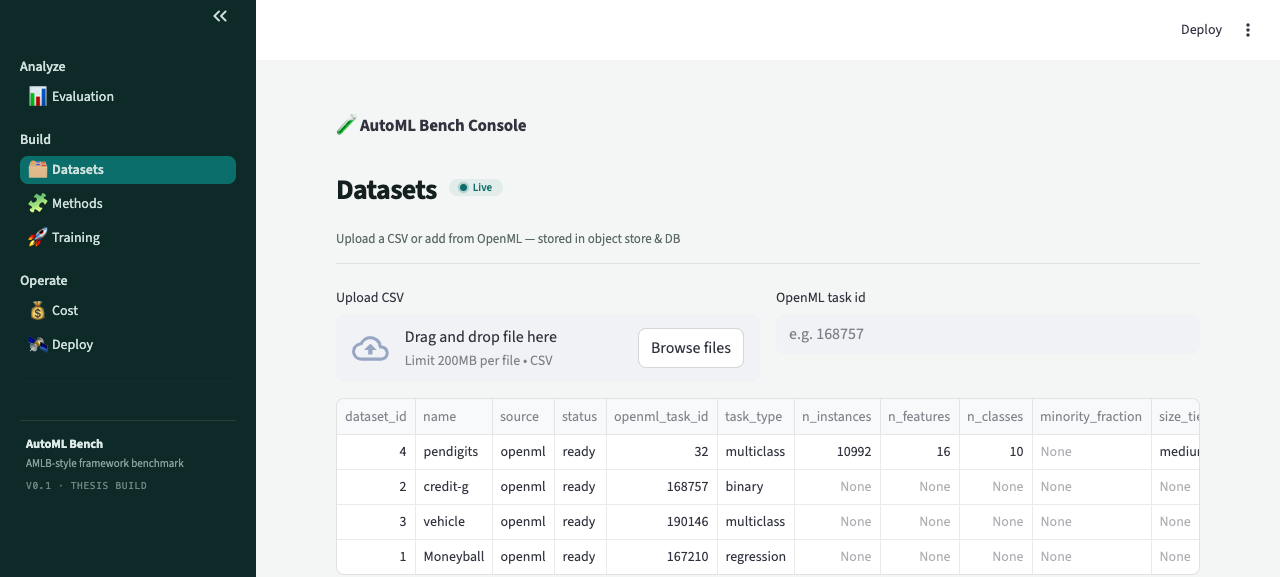
\includegraphics[width=0.88\linewidth]{image/console-datasets.png}
    \caption{Khu vực quản lý dữ liệu: nạp bộ dữ liệu từ tệp CSV, tác vụ OpenML
    hoặc liên kết Kaggle công khai.}
    \label{fig:console-datasets}
\end{figure}

Khu vực quản lý thư viện (Hình~\ref{fig:console-methods}) hiển thị danh mục các
thư viện AutoML kèm trạng thái tích hợp và mức độ tương thích với cấu hình máy
hiện tại. Trạng thái được báo cáo trung thực theo kết quả kiểm tra thực tế thay vì
giả định, nhờ đó người dùng biết trước thư viện nào có thể chạy được trên máy của
mình trước khi khởi động một lượt đánh giá kéo dài nhiều giờ.

\begin{figure}[H]
    \centering
    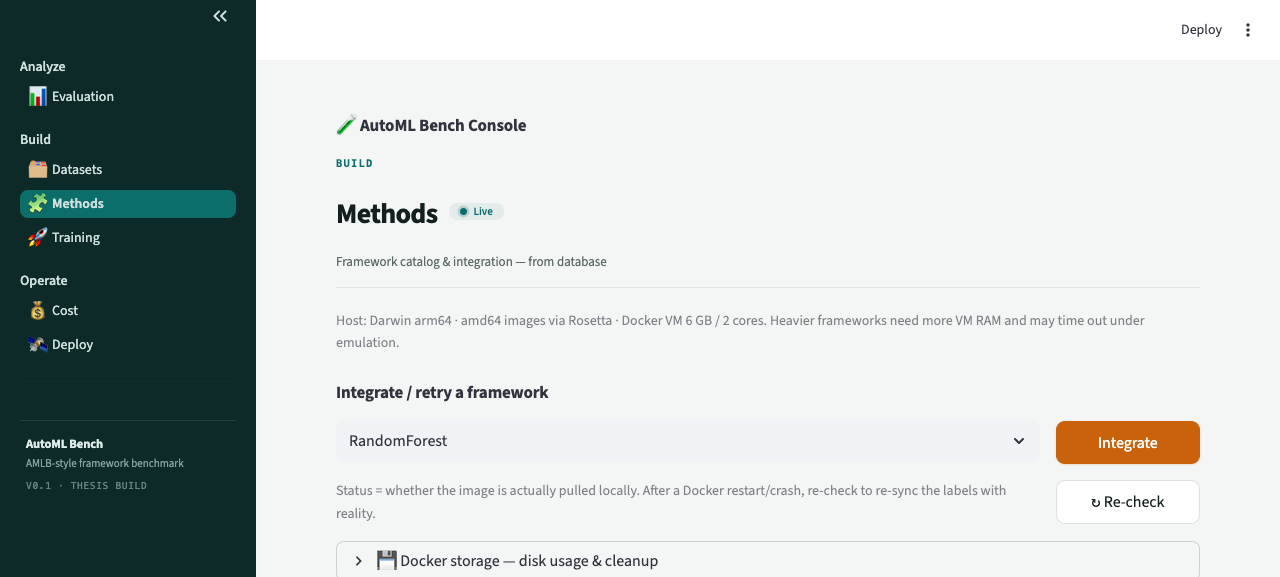
\includegraphics[width=0.88\linewidth]{image/console-methods.png}
    \caption{Khu vực quản lý thư viện: danh mục các thư viện AutoML kèm trạng thái
    tích hợp và phù hiệu tương thích theo cấu hình máy.}
    \label{fig:console-methods}
\end{figure}

Khu vực khởi chạy (Hình~\ref{fig:console-training}) cho phép chọn tổ hợp thư viện,
bộ dữ liệu và ngân sách thời gian, sau đó khởi động lượt đánh giá và theo dõi
trạng thái từng công việc theo thời gian thực. Cuối cùng, khu vực tổng hợp kết quả
(Hình~\ref{fig:console-eval}) trình bày bảng xếp hạng, biểu đồ đánh đổi giữa chất
lượng và thời gian, cùng khung nhìn phân tích theo đặc trưng bộ dữ liệu.

\begin{figure}[H]
    \centering
    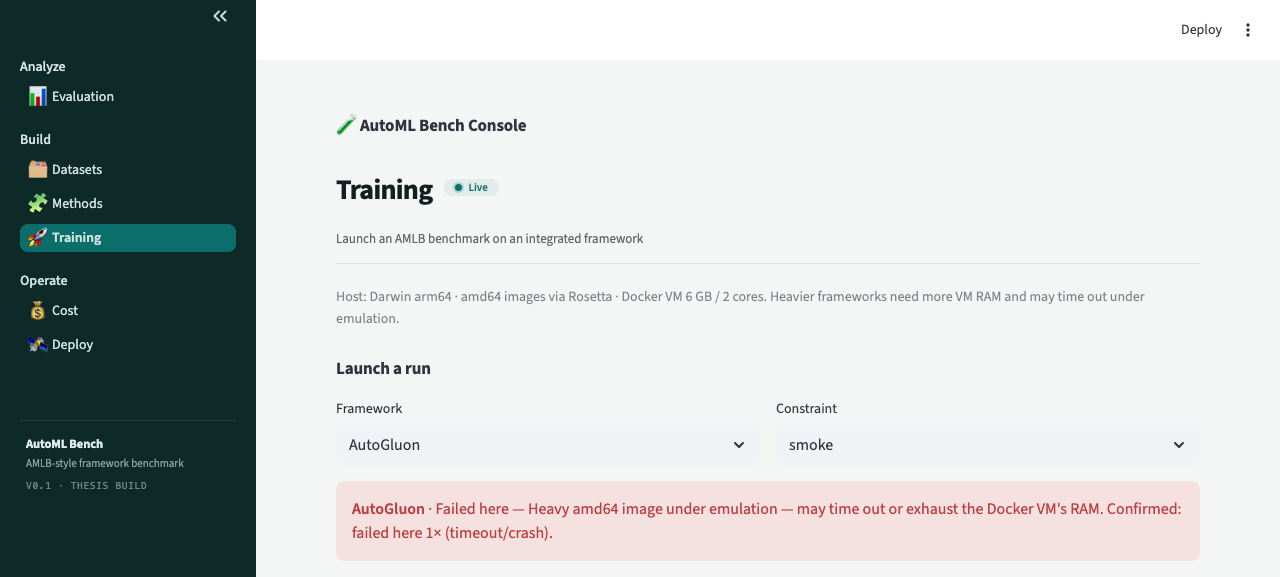
\includegraphics[width=0.88\linewidth]{image/console-training.png}
    \caption{Khu vực khởi chạy: lựa chọn thư viện, bộ dữ liệu và ngân sách thời
    gian, đồng thời theo dõi trạng thái các công việc đang thực thi.}
    \label{fig:console-training}
\end{figure}

\begin{figure}[H]
    \centering
    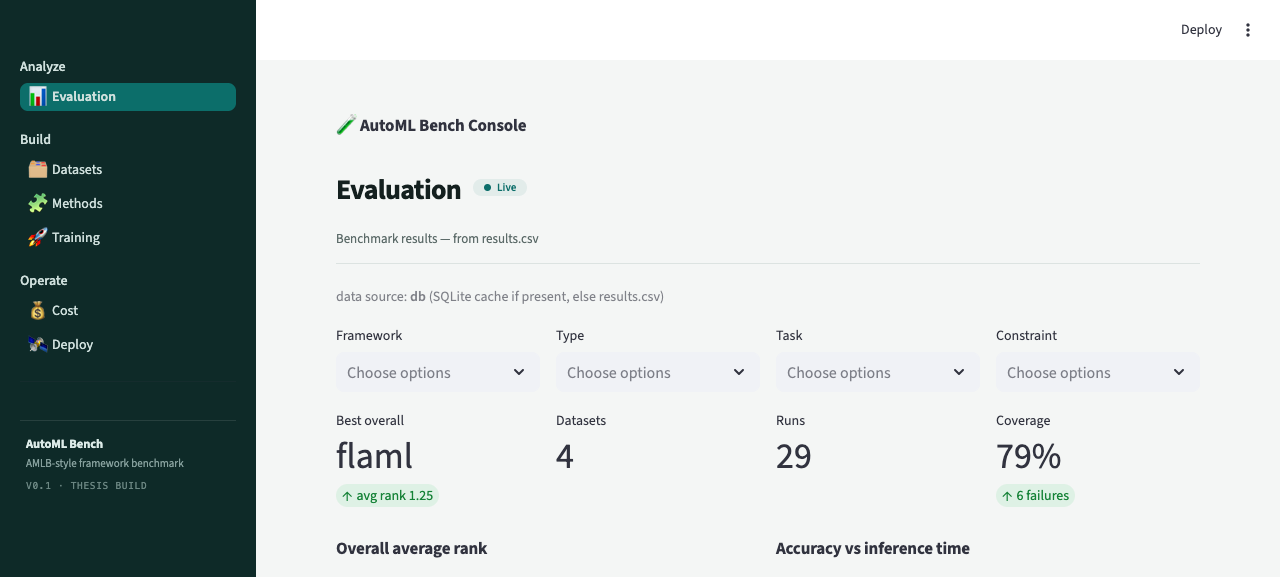
\includegraphics[width=0.88\linewidth]{image/eval-dashboard.png}
    \caption{Khu vực tổng hợp kết quả: bảng xếp hạng, biểu đồ đánh đổi chất lượng
    -- thời gian và khung nhìn theo đặc trưng bộ dữ liệu.}
    \label{fig:console-eval}
\end{figure}

Cần lưu ý rằng giao diện này đóng vai trò công cụ hỗ trợ khảo sát và trình diễn;
toàn bộ kết quả trình bày ở Chương~\ref{ch:thucnghiem} được tạo ra bằng bộ công cụ
dòng lệnh mô tả ở Mục~\ref{sec:kientruc}, vốn phù hợp hơn với việc chạy phân tán
trên nhiều máy trong thời gian dài.

\section{Thảo luận về các lựa chọn thiết kế}
\label{sec:thaoluan-pp}
Việc tách bạch giữa \emph{giao thức} và \emph{hiện thực} là lựa chọn thiết kế
trung tâm. Giao thức quy định các bất biến cần được bảo toàn để phép so sánh có
giá trị, còn hiện thực có thể thay đổi mà không ảnh hưởng tới tính đúng đắn của
kết luận.

Lựa chọn cô lập môi trường bằng môi trường ảo riêng cho từng thư viện, thay vì
đóng gói bằng container, xuất phát từ ràng buộc thực tế: khối lượng tính toán được
chia trên các máy cá nhân của thành viên nhóm cũng như trên nền tảng đám mây miễn
phí, nơi việc chạy container không phải lúc nào cũng khả dụng. Đánh đổi của lựa
chọn này là mức độ cô lập thấp hơn container ở tầng thư viện hệ thống; tuy nhiên,
vì mọi thư viện đều được đánh giá trên cùng một máy với cùng cấu hình phần cứng
trong mỗi lượt chạy, điều kiện công bằng theo Định nghĩa~\ref{def:congbang} vẫn
được bảo toàn.

Cơ chế khôi phục sau gián đoạn cũng là một yêu cầu bắt buộc chứ không phải tiện
ích phụ. Với thời gian chạy lên tới hàng chục giờ máy, xác suất gặp gián đoạn là
đáng kể; nếu không có khả năng tiếp tục từ điểm dừng, mỗi lần gián đoạn sẽ buộc
phải chạy lại từ đầu và làm cho thực nghiệm quy mô này trở nên bất khả thi.

Cuối cùng, quyết định giữ bước tiền xử lý ở mức tối thiểu phản ánh đúng mục tiêu
đánh giá. Nếu nhóm thực hiện mã hoá biến hạng mục hay điền giá trị khuyết một cách
công phu trước khi đưa vào các thư viện, phần năng lực xử lý dữ liệu thô --- vốn
là một thành phần quan trọng của AutoML --- sẽ bị che khuất, và kết quả so sánh
chỉ còn phản ánh năng lực tìm kiếm siêu tham số.

\section{Các yếu tố đe doạ tính hợp lệ và biện pháp kiểm soát}
\label{sec:hopleimuc}
Một thiết kế thực nghiệm chặt chẽ đòi hỏi nhận diện trước những yếu tố có thể làm
sai lệch kết luận. Bảng~\ref{tab:threats} liệt kê các yếu tố đã được nhóm nhận
diện cùng biện pháp kiểm soát tương ứng.

\begin{table}[H]
  \centering
  \small
  \caption{Các yếu tố đe doạ tính hợp lệ của kết luận và biện pháp kiểm soát.}
  \label{tab:threats}
  \renewcommand{\arraystretch}{1.25}
  \begin{tabularx}{\linewidth}{@{}>{\raggedright\arraybackslash}p{4.2cm} X@{}}
    \toprule
    \textbf{Yếu tố đe doạ} & \textbf{Biện pháp kiểm soát} \\
    \midrule
    Phương sai do phép chia dữ liệu &
    Phân hoạch fold sinh một lần từ hạt giống cố định, dùng chung cho mọi thư
    viện; phân tầng theo nhãn với bài toán phân loại. \\
    Xung đột phiên bản thư viện phụ thuộc &
    Mỗi thư viện được cài đặt và thực thi trong một môi trường ảo Python riêng
    biệt. \\
    Ngân sách tài nguyên không đồng nhất &
    Cùng một giá trị ngân sách được truyền vào tham số của mọi thư viện, kèm
    ngưỡng cứng do tiến trình cha áp đặt. \\
    Thiên lệch sống sót do bỏ qua thất bại &
    Mọi lần chạy đều sinh bản ghi; các lần thất bại được giữ lại kèm phân loại
    nguyên nhân và được phân tích riêng. \\
    Khác biệt phần cứng giữa các máy &
    Toàn bộ các thư viện trên cùng một bộ dữ liệu được chạy trên cùng một máy;
    việc phân tán được thực hiện theo chiều bộ dữ liệu chứ không cắt ngang một
    phép so sánh. \\
    Kết luận dựa trên chênh lệch không đáng kể &
    Báo cáo kèm độ lệch chuẩn giữa các fold; không tuyên bố hơn kém khi chênh
    lệch nằm dưới ngưỡng độ lệch chuẩn quan sát được. \\
    Thang đo khác nhau giữa các bộ dữ liệu &
    Xếp hạng dựa trên mô hình Bradley--Terry, vốn chỉ sử dụng quan hệ thứ tự nên
    bất biến với phép biến đổi đơn điệu của thang đo. \\
    \bottomrule
  \end{tabularx}
\end{table}

Yếu tố thứ năm trong bảng đáng được nhấn mạnh. Khi phân tán khối lượng tính toán
trên nhiều máy có cấu hình khác nhau, nếu chia việc theo chiều \emph{thư viện} thì
hai thư viện được so sánh có thể chạy trên hai máy khác nhau, và chênh lệch thời
gian quan sát được sẽ phản ánh sự khác biệt phần cứng chứ không phải thuật toán.
Vì vậy việc phân tán được thực hiện sao cho mọi thư viện trên cùng một bộ dữ liệu
luôn được đánh giá trên cùng một máy, giữ nguyên tính hợp lệ của phép so sánh
trong phạm vi từng bộ dữ liệu.

% ======================================================================
%  CHƯƠNG 4 — THỰC NGHIỆM VÀ PHÂN TÍCH KẾT QUẢ
%  Yêu cầu (mục 2.5): >= 2 bộ dữ liệu chuẩn; độ đo phù hợp; so sánh >= 2 baseline;
%  bảng + biểu đồ; phân tích; ablation study.
%  Lưu ý trung thực: các số liệu dưới đây là KẾT QUẢ SƠ BỘ (ngân sách 30s trên
%  máy cục bộ). Lần chạy đầy đủ trên 20 bộ dữ liệu (môi trường Docker/Linux) đang
%  được hoàn tất; các ô [ ] là chỗ điền số liệu cuối cùng.
%  Độ dài tham khảo: >= 10 trang.
% ======================================================================
\chapter{Thực nghiệm và phân tích kết quả}
\label{ch:thucnghiem}

\section{Bộ dữ liệu}
\label{sec:dulieu}
Đồ án sử dụng hai nhóm dữ liệu. \emph{Nhóm thứ nhất} là bộ sưu tập gồm 20 bộ dữ
liệu công khai thu thập từ Kaggle (mỗi thành viên chuẩn bị 5 bộ), cân bằng giữa
bài toán phân lớp và hồi quy, dùng cho lần chạy so sánh đầy đủ. \emph{Nhóm thứ
hai} là các bộ dữ liệu chuẩn nhỏ, dùng cho lần chạy sơ bộ nhằm kiểm chứng quy
trình end-to-end. Bảng~\ref{tab:dulieu} thống kê ba bộ dữ liệu của lần chạy sơ bộ.
Việc nạp và quản lý dữ liệu được thực hiện qua giao diện của hệ thống
(Hình~\ref{fig:console-datasets}).

\begin{figure}[H]
    \centering
    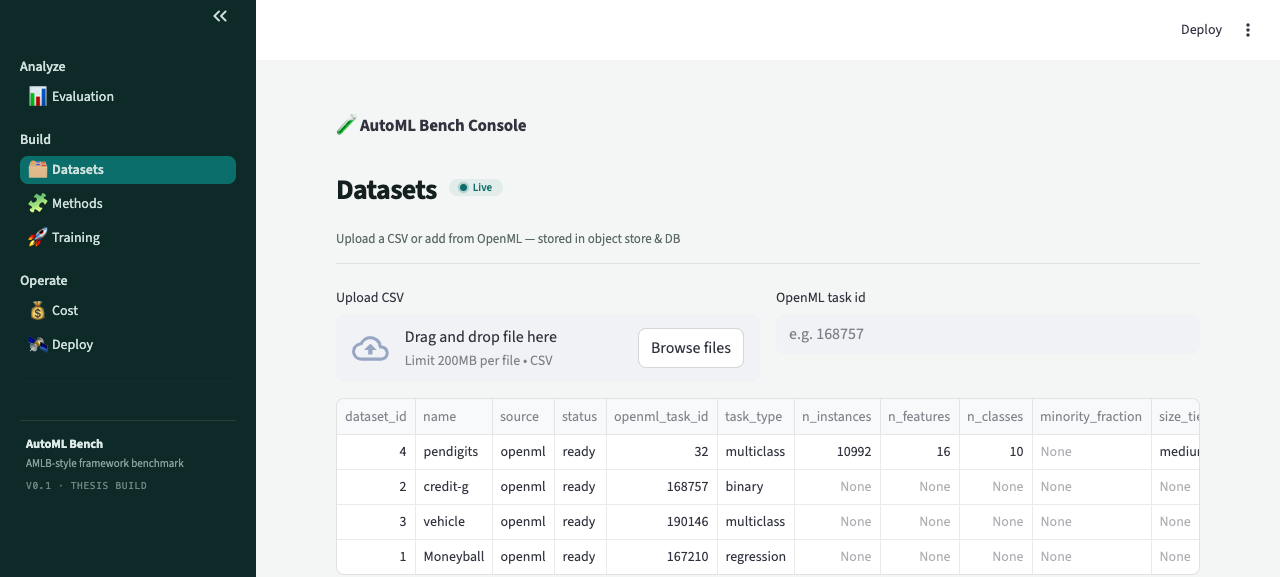
\includegraphics[width=0.9\linewidth]{image/console-datasets.png}
    \caption{Trang Datasets: nạp dữ liệu từ tệp CSV, tác vụ OpenML hoặc liên kết
    Kaggle công khai; mỗi bộ được ghi nhận kèm loại, nguồn và trạng thái.}
    \label{fig:console-datasets}
\end{figure}

\begin{table}[H]
  \centering
  \small
  \caption{Ba bộ dữ liệu dùng trong lần chạy sơ bộ.}
  \label{tab:dulieu}
  \renewcommand{\arraystretch}{1.2}
  \begin{tabularx}{\linewidth}{@{}l l l X@{}}
    \toprule
    \textbf{Bộ dữ liệu} & \textbf{Loại tác vụ} & \textbf{Độ đo} & \textbf{Ghi chú} \\
    \midrule
    breast\_cancer       & Phân lớp nhị phân & AUC       & Chẩn đoán u lành/ác. \\
    wine                 & Phân lớp đa lớp   & log-loss  & Phân loại ba giống rượu vang. \\
    california\_housing  & Hồi quy           & RMSE      & Dự đoán giá nhà. \\
    \bottomrule
  \end{tabularx}
\end{table}

\noindent Bảng~\ref{tab:dulieu-full} là khung thống kê cho bộ 20 bộ dữ liệu Kaggle
(điền khi hoàn tất thu thập).

\begin{table}[H]
  \centering
  \small
  \caption{Thống kê bộ 20 bộ dữ liệu Kaggle (khung điền).}
  \label{tab:dulieu-full}
  \renewcommand{\arraystretch}{1.15}
  \begin{tabularx}{\linewidth}{@{}l c c c X@{}}
    \toprule
    \textbf{Bộ dữ liệu} & \textbf{Tác vụ} & \textbf{Số mẫu} & \textbf{Số đặc trưng} & \textbf{Nguồn} \\
    \midrule
    {[}\ldots{]} & {[}\ldots{]} & {[}\ldots{]} & {[}\ldots{]} & Kaggle: {[}liên kết{]} \\
    \multicolumn{5}{c}{\textit{\ldots\ (tổng cộng 20 bộ: 10 phân lớp, 10 hồi quy)}} \\
    \bottomrule
  \end{tabularx}
\end{table}

\section{Thiết lập thực nghiệm}
\label{sec:thietlap}
\textbf{Thư viện so sánh:} FLAML, H2O~AutoML và AutoGluon. \\
\textbf{Baseline:} rừng ngẫu nhiên (\textit{RandomForest}) và bộ dự đoán hằng
(\textit{constantpredictor}) --- hai baseline được AMLB cung cấp sẵn, dùng làm mốc
dưới để kiểm tra xem một thư viện có thực sự ``học'' được gì hay không. \\
\textbf{Ràng buộc tài nguyên:} theo ba mức của AMLB --- \texttt{smoke} (1 fold,
60 giây, 4 nhân), \texttt{1h} (10 fold, 3600 giây, 8 nhân) và \texttt{4h} (10
fold, 14400 giây, 8 nhân). Lần chạy sơ bộ dùng ngân sách 30 giây/fold. \\
\textbf{Môi trường:} mỗi thư viện chạy trong ảnh Docker \texttt{automlbenchmark/*}
riêng để bảo đảm môi trường đồng nhất; siêu dữ liệu và kết quả lưu trên
PostgreSQL, tệp dữ liệu và dự đoán lưu trên MinIO. Người dùng chọn thư viện, bộ
dữ liệu và ngân sách rồi khởi chạy trực tiếp từ trang Training
(Hình~\ref{fig:console-training}).

\begin{figure}[H]
    \centering
    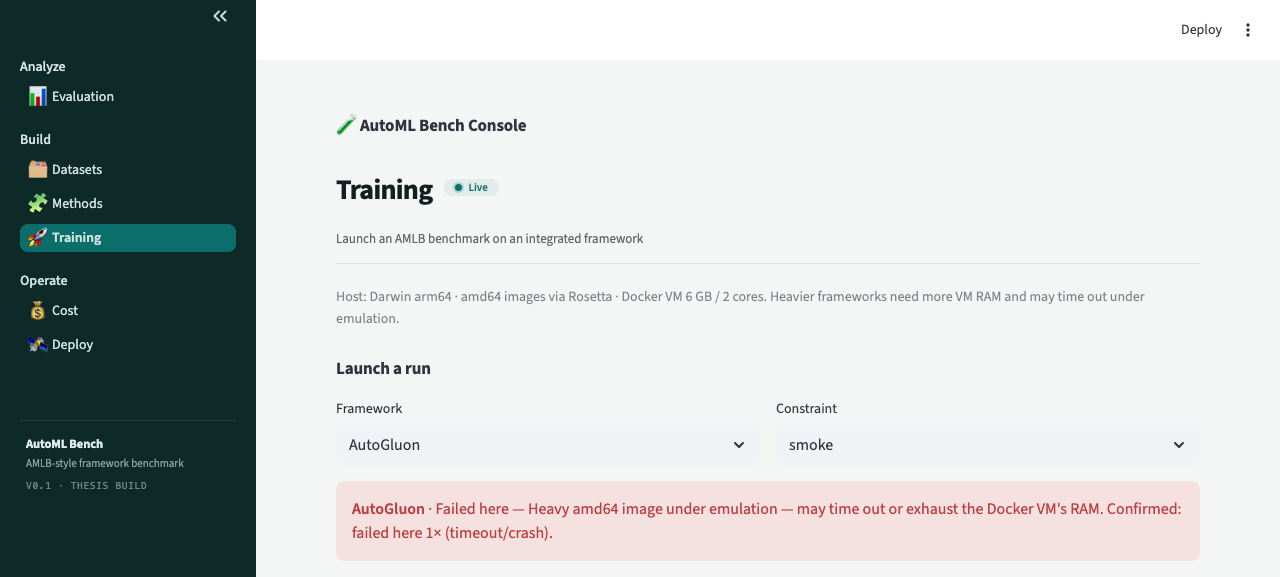
\includegraphics[width=0.9\linewidth]{image/console-training.png}
    \caption{Trang Training: chọn thư viện, bộ dữ liệu và ngân sách để khởi chạy
    một lần đánh giá trong Docker; các tác vụ tự động cập nhật trạng thái.}
    \label{fig:console-training}
\end{figure}

\section{Độ đo đánh giá}
\label{sec:dodo}
Nhóm dùng AUC cho phân lớp nhị phân, log-loss cho phân lớp đa lớp và RMSE cho hồi
quy (định nghĩa và ví dụ tính đã trình bày ở Mục~\ref{sec:dodo-lythuyet}, Ví
dụ~\ref{vd:rmse}). Kết quả tổng hợp được quy về \emph{thứ hạng trung bình} theo
công thức ở Mục~\ref{sec:giaothuc} để so sánh xuyên suốt các loại độ đo.

\section{Kết quả sơ bộ và xếp hạng}
\label{sec:ketqua}
Bảng~\ref{tab:ketqua} trình bày điểm số và chi phí thời gian của ba thư viện trên
ba bộ dữ liệu ở ngân sách 30 giây/fold. Đây là kết quả \emph{sơ bộ} nhằm kiểm
chứng quy trình; lần chạy đầy đủ trên 20 bộ dữ liệu đang được hoàn tất.

\begin{table}[H]
  \centering
  \small
  \caption{Kết quả sơ bộ: điểm số (và thời gian chạy, giây) ở ngân sách 30s/fold.
  Giá trị tốt nhất mỗi hàng được in đậm.}
  \label{tab:ketqua}
  \renewcommand{\arraystretch}{1.25}
  \begin{tabularx}{\linewidth}{@{}>{\raggedright\arraybackslash}X c c c@{}}
    \toprule
    \textbf{Bộ dữ liệu (độ đo)} & \textbf{FLAML} & \textbf{AutoGluon} & \textbf{H2O} \\
    \midrule
    breast\_cancer (AUC $\uparrow$)
        & \makecell{0.9957\\(68.2s)} & \makecell{0.9961\\(37.4s)} & \makecell{\textbf{0.9974}\\(57.4s)} \\
    california\_housing (RMSE $\downarrow$)
        & \makecell{0.4693\\(33.8s)} & \makecell{\textbf{0.4320}\\(31.5s)} & \makecell{0.4389\\(125.9s)} \\
    wine (log-loss $\downarrow$)
        & \makecell{0.0487\\(161.4s)} & \makecell{0.0099\\(31.5s)} & \makecell{\textbf{0.0038}\\(130.7s)} \\
    \midrule
    \textbf{Thứ hạng trung bình} & 3.00 & 1.67 & \textbf{1.33} \\
    \bottomrule
  \end{tabularx}
\end{table}

Cách tính thứ hạng trung bình đã được minh hoạ ở Ví dụ~\ref{vd:rank}. Hình
\ref{fig:rank} trực quan hoá thứ hạng này (thấp hơn là tốt hơn).

\begin{figure}[H]
    \centering
    \begin{tikzpicture}
    \begin{axis}[
        width=0.72\linewidth, height=5.2cm,
        ybar, bar width=20pt,
        symbolic x coords={H2O, AutoGluon, FLAML},
        xtick=data, ymin=0, ymax=3.4,
        ylabel={Thứ hạng TB ($\downarrow$)},
        nodes near coords, enlarge x limits=0.35]
      \addplot coordinates {(H2O, 1.33) (AutoGluon, 1.67) (FLAML, 3.00)};
    \end{axis}
    \end{tikzpicture}
    \caption{Thứ hạng trung bình của ba thư viện trên lần chạy sơ bộ (càng thấp
    càng tốt).}
    \label{fig:rank}
\end{figure}

Ở ngân sách nhỏ này, H2O và AutoGluon nhỉnh hơn FLAML về chất lượng, nhưng FLAML
và AutoGluon thường hoàn tất nhanh hơn --- cho thấy sự \emph{đánh đổi giữa chất
lượng và thời gian}. Bảng~\ref{tab:full} là khung tổng hợp cho lần chạy đầy đủ.

\begin{table}[H]
  \centering
  \small
  \caption{Kết quả tổng hợp trên 20 bộ dữ liệu (khung điền cho lần chạy đầy đủ).}
  \label{tab:full}
  \renewcommand{\arraystretch}{1.2}
  \begin{tabularx}{\linewidth}{@{}X c c c c@{}}
    \toprule
    \textbf{Thư viện} & \textbf{Thắng phân lớp} & \textbf{Thắng hồi quy} & \textbf{Thứ hạng TB} & \textbf{Thời gian TB} \\
    \midrule
    FLAML      & [\,] & [\,] & [\,] & [\,] \\
    H2O AutoML & [\,] & [\,] & [\,] & [\,] \\
    AutoGluon  & [\,] & [\,] & [\,] & [\,] \\
    RandomForest (baseline)     & [\,] & [\,] & [\,] & [\,] \\
    constantpredictor (baseline)& [\,] & [\,] & [\,] & [\,] \\
    \bottomrule
  \end{tabularx}
\end{table}

\section{So sánh với baseline}
\label{sec:baseline}
Theo giao thức AMLB, mọi thư viện được đối chiếu với hai baseline. Một thư viện
AutoML chỉ thực sự có giá trị nếu vượt rõ rệt bộ dự đoán hằng và ít nhất không
thua rừng ngẫu nhiên. [Điền phân tích sau lần chạy đầy đủ: thư viện nào vượt
baseline trên loại tác vụ nào, mức vượt bao nhiêu.]

\section{Nghiên cứu loại bỏ thành phần (ablation)}
\label{sec:ablation}
Nhóm khảo sát ảnh hưởng của \emph{ngân sách thời gian} --- yếu tố tác động mạnh
tới AutoML --- bằng cách chạy cùng cấu hình ở các mức ngân sách khác nhau và quan
sát biến thiên của chất lượng và thứ hạng (Bảng~\ref{tab:ablation}).

\begin{table}[H]
  \centering
  \small
  \caption{Ablation theo ngân sách thời gian (thứ hạng trung bình).}
  \label{tab:ablation}
  \renewcommand{\arraystretch}{1.2}
  \begin{tabular}{@{}lccc@{}}
    \toprule
    \textbf{Ngân sách} & \textbf{FLAML} & \textbf{AutoGluon} & \textbf{H2O} \\
    \midrule
    30 giây/fold (sơ bộ) & 3.00 & 1.67 & 1.33 \\
    smoke (60s, 1 fold)  & [\,] & [\,] & [\,] \\
    1h (3600s, 10 fold)  & [\,] & [\,] & [\,] \\
    \bottomrule
  \end{tabular}
\end{table}

[Phân tích: khi tăng ngân sách, thứ hạng giữa các thư viện thay đổi ra sao; thư
viện nào tận dụng ngân sách lớn tốt hơn.]

\section{Phân tích lỗi và thảo luận}
\label{sec:phantichloi}
Việc ghi nhận thất bại (thay vì bỏ qua) giúp phân tích các nguyên nhân thực tế
cản trở một so sánh công bằng. Trên máy cục bộ macOS (arm64, Python~3.9), nhóm
quan sát các lỗi sau khi cố gắng chạy trực tiếp không dùng Docker:
\begin{itemize}
    \item \textbf{Lệch phiên bản thư viện phụ thuộc:} \texttt{TunedRandomForest}
    lỗi do \texttt{scikit-learn 1.6.1} đã loại bỏ hàm \texttt{\_check\_fit\_params}
    mà AMLB còn gọi --- một minh hoạ điển hình cho việc môi trường không đồng nhất
    phá vỡ tính tái lập.
    \item \textbf{Thiếu thư viện hệ thống:} FLAML cần \texttt{libomp} cho XGBoost
    (khắc phục bằng cách cài đặt bổ sung).
    \item \textbf{Kịch bản cài đặt hướng Linux:} H2O và AutoGluon dùng script cài
    đặt cho Linux, thất bại trên macOS (\texttt{AutoGluon setup.sh} thoát mã 127).
\end{itemize}
Bốn trong sáu bộ chạy thất bại khi chạy cục bộ. Quan sát này chính là lý do đồ án
chọn chạy lần đánh giá đầy đủ trong \emph{môi trường Docker/Linux đồng nhất}: chỉ
khi cô lập môi trường thì so sánh giữa H2O, FLAML và AutoGluon mới thực sự công
bằng. Hình~\ref{fig:console-methods} minh hoạ trang quản lý và tích hợp thư viện
của hệ thống, nơi trạng thái tích hợp và mức tương thích theo máy được hiển thị
trung thực.

\begin{figure}[H]
    \centering
    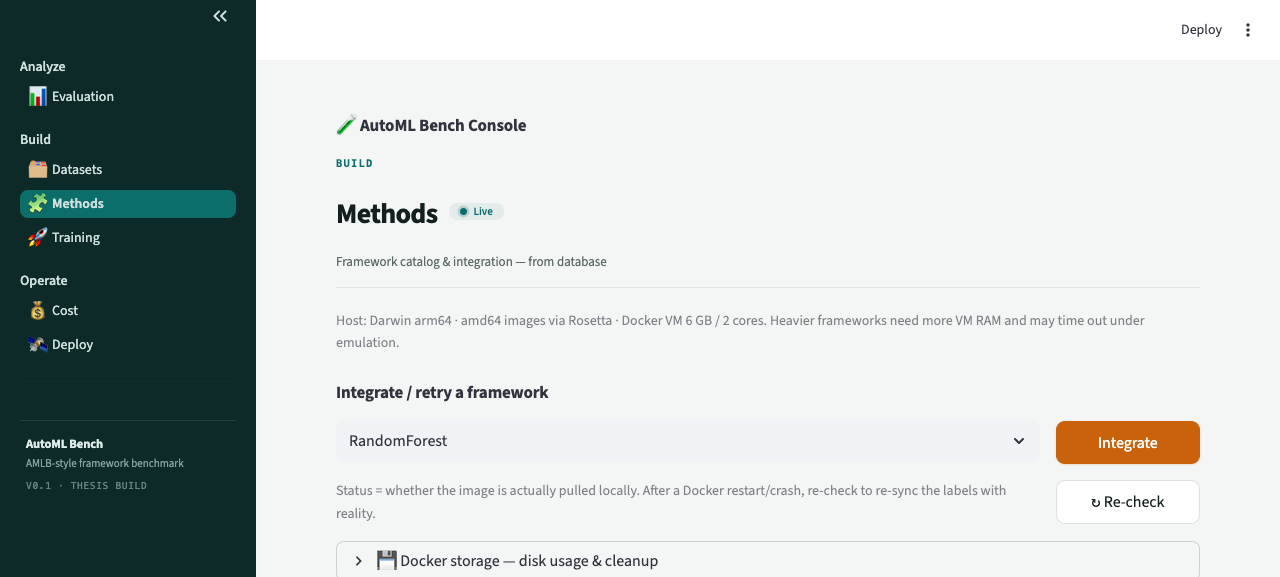
\includegraphics[width=0.9\linewidth]{image/console-methods.png}
    \caption{Trang Methods: danh mục thư viện AutoML với trạng thái tích hợp, phù
    hiệu tương thích theo máy và dung lượng Docker.}
    \label{fig:console-methods}
\end{figure}

Tổng hợp lại, kết quả sơ bộ đã kiểm chứng quy trình end-to-end (chạy $\to$ chấm
điểm $\to$ xếp hạng) dưới một giao thức thống nhất; phần phân tích lỗi cho thấy
giá trị của việc ghi nhận thất bại và cô lập môi trường. Kết quả đầy đủ trên 20
bộ dữ liệu sẽ củng cố các nhận định về sự đánh đổi chất lượng -- chi phí giữa các
thư viện.

% ======================================================================
%  CHƯƠNG 5 — KẾT LUẬN VÀ HƯỚNG PHÁT TRIỂN TƯƠNG LAI
% ======================================================================
\chapter{Kết luận và hướng phát triển tương lai}
\label{ch:ketluan}

\section{Kết luận}
\label{sec:ketluan}
Đồ án đã xây dựng và vận hành một quy trình đánh giá công bằng cho các thư viện
học máy tự động, đồng thời áp dụng quy trình đó để so sánh bốn thư viện AutoML mã
nguồn mở trên 12 bộ dữ liệu thực thu thập từ Kaggle.

Về mặt phương pháp luận, đồ án đã hệ thống hoá bốn điều kiện của một phép so sánh
công bằng và hiện thực hoá từng điều kiện bằng một cơ chế kiểm soát cụ thể: phân
hoạch fold được sinh một lần từ hạt giống cố định và dùng chung cho mọi thư viện;
mỗi thư viện được cô lập trong một môi trường ảo riêng nhằm loại trừ xung đột phụ
thuộc; ngân sách thời gian được áp đặt đồng nhất ở cả hai lớp thư viện và tiến
trình; và mọi lần chạy thất bại đều được ghi nhận kèm phân loại nguyên nhân thay
vì bị loại khỏi thống kê.

Về mặt hạ tầng, nhóm đã xây dựng bộ công cụ điều phối theo mô hình tiến trình chủ
--- tiến trình con, hỗ trợ phân tán khối lượng tính toán trên nhiều máy, khôi phục
sau gián đoạn và hợp nhất kết quả từng phần. Hạ tầng này đã hoàn tất khối lượng
thực nghiệm gồm bốn thư viện trên 12 bộ dữ liệu với 5 fold và hai mức ngân sách
thời gian.

Về mặt kết quả, phát hiện quan trọng nhất là \emph{không tồn tại thư viện AutoML
vượt trội toàn diện}. Mô hình cây Bradley--Terry cho thấy thứ hạng đảo chiều rõ
rệt giữa các dạng tác vụ: H2O~AutoML dẫn đầu ở phân loại đa lớp và hồi quy nhưng
xếp cuối ở phân loại nhị phân, trong khi MLJAR đứng đầu nhóm nhị phân nhưng xếp
cuối nhóm đa lớp. Một xếp hạng toàn cục đơn lẻ, nếu được sử dụng, sẽ che khuất
hoàn toàn cấu trúc này.

Bên cạnh đó, thực nghiệm cho thấy chênh lệch về chất lượng dự đoán giữa các thư
viện thường nhỏ hơn độ lệch chuẩn giữa các fold, trong khi chênh lệch về chi phí
tài nguyên lại rất lớn: thời gian huấn luyện chênh nhau tới bốn lần và bộ nhớ tới
hơn mười lần cho cùng một mức chất lượng. Điều này gợi ý rằng trong thực tiễn
triển khai, các tiêu chí về chi phí, độ ổn định và tỉ lệ thất bại nên được cân
nhắc ngang bằng, nếu không muốn nói là trước, so với chỉ số chất lượng thuần tuý.

\section{Trả lời các câu hỏi nghiên cứu}
\label{sec:traloi}
Đối chiếu với mục tiêu đặt ra ở Chương~\ref{ch:gioithieu}, các kết quả thu được
cho phép trả lời ba câu hỏi trung tâm của đồ án.

\paragraph{Có tồn tại một thư viện AutoML tốt nhất hay không?} Câu trả lời là
không. Mô hình cây Bradley--Terry cho thấy H2O~AutoML đạt cường độ $0.446$ ở nhóm
phân loại đa lớp và $0.389$ ở nhóm hồi quy --- dẫn đầu cả hai --- nhưng chỉ đạt
$0.164$ ở nhóm phân loại nhị phân, tức xếp cuối. MLJAR thể hiện xu hướng ngược
lại. Nếu chỉ nhìn vào bảng xếp hạng toàn cục, nơi ba thư viện dẫn đầu chênh nhau
chưa tới $0.03$, cấu trúc đảo chiều này sẽ hoàn toàn bị che khuất. Kết luận rút ra
là việc lựa chọn thư viện phải xuất phát từ dạng tác vụ cụ thể, và các bảng xếp
hạng AutoML rút gọn thành một con số duy nhất cần được tiếp nhận thận trọng.

\paragraph{Chênh lệch giữa các thư viện nằm ở đâu?} Không nằm chủ yếu ở chất lượng
dự đoán. Trên nhiều bộ dữ liệu, khác biệt điểm số giữa thư viện tốt nhất và kém
nhất nhỏ hơn độ lệch chuẩn giữa các fold của chính từng thư viện --- trường hợp
\texttt{adult\_income} với chênh lệch AUC $0.0018$ so với độ lệch chuẩn
$0.0015$--$0.0019$ là ví dụ điển hình. Trong khi đó, chênh lệch về thời gian huấn
luyện lên tới bốn lần và về bộ nhớ lên tới hơn mười lần. Do vậy, trong phần lớn
tình huống ứng dụng, tiêu chí chi phí và độ ổn định có sức phân biệt cao hơn tiêu
chí chất lượng.

\paragraph{Cấp thêm tài nguyên có luôn cải thiện kết quả không?} Không phải lúc
nào cũng vậy. Khi tăng ngân sách từ $60$ lên $300$ giây, MLJAR cải thiện mạnh về
chất lượng (từ $0.59$ lên $0.79$ trên thang chuẩn hoá) nhưng đồng thời tăng tỉ lệ
thất bại từ $0\%$ lên khoảng $20\%$. Việc nới lỏng ràng buộc thời gian đã kích
hoạt các chế độ tìm kiếm tốn bộ nhớ hơn, qua đó chuyển nút thắt cổ chai từ thời
gian sang bộ nhớ. Quan hệ giữa tài nguyên và hiệu năng, vì vậy, không đơn điệu và
cần được kiểm soát đồng thời trên nhiều chiều.

\section{Giới hạn của nghiên cứu}
\label{sec:hanche}
Nhóm ghi nhận một số giới hạn của kết quả trình bày trong báo cáo.

\textbf{Về phép đo bộ nhớ.} Mức tiêu thụ bộ nhớ được quan sát từ tiến trình
Python, do đó không phản ánh đúng thực tế đối với H2O~AutoML --- thư viện thực
hiện huấn luyện trong một tiến trình máy ảo Java riêng biệt. Vì lý do này, đồ án
không xếp hạng các thư viện theo tiêu chí bộ nhớ, và các con số của H2O ở
Mục~\ref{sec:bonho} chỉ nên được hiểu là chi phí phía máy khách.

\textbf{Về tuyến phương pháp cơ sở.} Đây là giới hạn đáng kể nhất của nghiên cứu.
Trong tổng số 120 lần chạy đã lên lịch cho hai phương pháp cơ sở, chỉ 15 lần hoàn
tất; phần còn lại hoặc dừng giữa chừng, hoặc chưa được thực thi do quỹ thời gian
tính toán mà nhóm huy động được đã dùng gần hết cho bốn thư viện AutoML chính.
Riêng rừng ngẫu nhiên còn vướng một khiếm khuyết ở lớp bao phương pháp cơ sở như
đã nêu ở Mục~\ref{sec:baseline}. Hệ quả là đối chiếu ở Bảng~\ref{tab:baseline}
mới thực hiện được với một phương pháp cơ sở trên ba bộ dữ liệu, thay vì hai
phương pháp trên toàn bộ mười hai bộ như thiết kế ban đầu.

\textbf{Về quy mô ngân sách.} Thực nghiệm giới hạn ở hai mức ngân sách $60$ và
$300$ giây. Các nghiên cứu quy mô lớn thường sử dụng ngân sách hàng giờ, nơi trật
tự giữa các thư viện có thể thay đổi --- đặc biệt với những thư viện còn nhiều dư
địa cải thiện như MLJAR.

\textbf{Về mức độ cô lập môi trường.} Bộ kết quả trong báo cáo được tạo bằng đường
dòng lệnh, vốn cô lập các thư viện ở mức môi trường ảo Python. Lựa chọn này cho
phép chạy phân tán trên nhiều máy nhưng không cô lập tầng thư viện hệ thống như
container. Điều kiện công bằng vẫn được bảo toàn trong mỗi lượt chạy vì mọi thư
viện dùng chung một cấu hình phần cứng; đổi lại, việc tái lập chính xác trên máy
khác đòi hỏi thêm thao tác thiết lập. Đường chạy trên nền Docker của AMLB Studio
khắc phục hạn chế này nhưng chưa được dùng cho lượt đánh giá hiện tại.

\textbf{Về ý nghĩa thống kê.} Các chênh lệch nhỏ giữa những thư viện dẫn đầu chưa
được kiểm chứng bằng kiểm định hình thức. Báo cáo đã thận trọng không tuyên bố
thắng thua khi chênh lệch nằm dưới ngưỡng độ lệch chuẩn giữa các fold, nhưng đây
là biện pháp phòng vệ chứ không thay thế được một kiểm định đúng nghĩa.

\textbf{Về phạm vi bài toán.} Nghiên cứu giới hạn ở dữ liệu dạng bảng với ba dạng
tác vụ học có giám sát; các kết luận không mở rộng trực tiếp sang dữ liệu ảnh, văn
bản hay chuỗi thời gian.

\section{Hướng phát triển tương lai}
\label{sec:huongphattrien}

\subsection{Hoàn tất tuyến phương pháp cơ sở}
Như đã ghi nhận ở Mục~\ref{sec:baseline}, tuyến phương pháp cơ sở chưa chạy trọn
vẹn do quỹ thời gian tính toán của nhóm đã dành phần lớn cho bốn thư viện AutoML
chính, và riêng rừng ngẫu nhiên còn vướng lỗi mã hoá dữ liệu đầu vào. Khắc phục
không đòi hỏi thay đổi giao thức mà chỉ cần hai việc: bổ sung một bước tiền xử lý
tối thiểu và đồng nhất --- mã hoá one-hot cho biến hạng mục, điền giá trị khuyết
bằng trung vị --- vào lớp bao phương pháp cơ sở, rồi chạy lại trên toàn bộ 12 bộ
dữ liệu. Chi phí tính toán cho bước này thấp hơn nhiều so với một lượt chạy AutoML,
bởi cả hai phương pháp cơ sở đều không thực hiện tìm kiếm siêu tham số.

Giá trị của việc này vượt xa một dòng số liệu bổ sung. Rừng ngẫu nhiên với cấu
hình mặc định là ngưỡng so sánh có ý nghĩa thực tiễn nhất trong toàn bộ nghiên
cứu: nó lượng hoá phần lợi ích mà quá trình tìm kiếm tự động mang lại so với
phương án đơn giản nhất mà một người thực hành có kinh nghiệm sẽ chọn. Nếu khoảng
cách đó hẹp trên phần lớn bộ dữ liệu, kết luận thực tiễn của đề tài sẽ thay đổi
đáng kể --- và đó là câu hỏi mà bộ kết quả hiện tại chưa trả lời được.

\subsection{Áp dụng kiểm định thống kê lên bộ kết quả hiện có}
Quy trình kiểm định Friedman và hậu kiểm Nemenyi đã được hiện thực trong lớp phân
tích của hệ thống (Mục~\ref{sec:console}) nhưng chưa được áp dụng lên bộ kết quả ở
Chương~\ref{ch:thucnghiem}, do hai phần được phát triển song song trên hai nhánh
khác nhau. Kết nối chúng là bước tiếp theo trực tiếp nhất và không đòi hỏi chạy
lại thực nghiệm.

Với bốn thư viện trên 12 bộ dữ liệu, sau khi thu về tập con đầy đủ vẫn còn chín bộ,
vượt ngưỡng tối thiểu mà kiểm định yêu cầu. Kết quả sẽ cho phép phát biểu dứt khoát
hai điều mà báo cáo hiện chỉ nhận định dựa trên độ lệch chuẩn quan sát: cách biệt
giữa H2O và FLAML ở nhóm hồi quy có phải khác biệt thực hay không, và khoảng cách
$0.004$ giữa H2O và MLJAR ở mức toàn cục có nằm dưới ngưỡng phân biệt hay không.
Biểu đồ khoảng cách tới hạn đi kèm sẽ thay cách trình bày thứ hạng hiện tại bằng
một hình thức chặt chẽ hơn, trong đó những thư viện không phân biệt được về mặt
thống kê được nối với nhau thay vì bị xếp thứ tự dứt khoát.

\subsection{Mở rộng thang ngân sách và khảo sát đường cong hội tụ}
Thay vì chỉ so sánh hai mức ngân sách rời rạc, hướng phát triển tiếp theo là ghi
nhận đường cong hiệu năng theo thời gian trong suốt quá trình tìm kiếm của mỗi thư
viện. Cách tiếp cận này cho phép trả lời những câu hỏi mà thiết kế hiện tại chưa
xử lý được: mỗi thư viện cần bao nhiêu thời gian để đạt $95\%$ hiệu năng cuối
cùng, và thời điểm nào hiệu suất biên của việc cấp thêm tài nguyên trở nên không
đáng kể. Với kết quả cho thấy MLJAR cải thiện mạnh từ $0.59$ lên $0.79$ khi tăng
ngân sách, việc xác định điểm bão hoà của thư viện này có giá trị thực tiễn trực
tiếp trong việc hoạch định tài nguyên.

\subsection{Kiểm soát đồng thời nhiều chiều tài nguyên}
Phát hiện về việc MLJAR tăng tỉ lệ thất bại khi được cấp thêm thời gian cho thấy
ngân sách thời gian và ngân sách bộ nhớ tương tác với nhau theo cách không hiển
nhiên. Hướng nghiên cứu tiếp theo là thiết kế thực nghiệm hai chiều, trong đó cả
giới hạn thời gian lẫn giới hạn bộ nhớ đều được biến thiên có hệ thống, nhằm xây
dựng bản đồ vùng vận hành an toàn cho từng thư viện. Kết quả sẽ trả lời câu hỏi
mà người triển khai thực sự quan tâm: với một cấu hình máy cho trước, mức ngân
sách thời gian nào là tối ưu mà vẫn giữ tỉ lệ thất bại ở mức chấp nhận được.

\subsection{Đo bộ nhớ ở mức tiến trình hệ điều hành}
Để khắc phục giới hạn của phép đo hiện tại, mức tiêu thụ bộ nhớ nên được ghi nhận
ở mức tiến trình hệ điều hành thay vì từ bên trong tiến trình Python, qua đó bao
gồm cả bộ nhớ do máy ảo Java của H2O cấp phát. Khi đó, bộ nhớ mới có thể trở thành
một tiêu chí xếp hạng hợp lệ bên cạnh chất lượng và thời gian, và bức tranh đánh
đổi giữa các thư viện sẽ hoàn chỉnh hơn.

\subsection{Tích hợp meta-learning để khuyến nghị tự động}
Kết quả của đồ án cho thấy thư viện phù hợp phụ thuộc vào dạng tác vụ và đặc điểm
dữ liệu. Điều này gợi mở khả năng xây dựng một cơ chế khuyến nghị tự động: từ các
đặc trưng mô tả bộ dữ liệu (số mẫu, số đặc trưng, tỉ lệ biến hạng mục, mức mất cân
bằng nhãn, dạng tác vụ), huấn luyện một mô hình dự đoán thư viện nào có khả năng
cho kết quả tốt nhất trong ngân sách cho trước. Bộ kết quả gồm 12 bộ dữ liệu hiện
tại còn quá nhỏ để huấn luyện một mô hình như vậy, song việc mở rộng tập dữ liệu
lên vài chục bộ sẽ tạo đủ cơ sở. Hướng phát triển này biến kết quả đánh giá từ một
bảng tra cứu tĩnh thành một công cụ hỗ trợ ra quyết định.

\subsection{Mở rộng tập thư viện và dạng dữ liệu}
Cuối cùng, việc bổ sung các thư viện theo hướng tiếp cận khác biệt --- chẳng hạn
auto-sklearn với tối ưu Bayes kết hợp meta-learning, hay TPOT với giải thuật tiến
hoá --- sẽ giúp kiểm chứng liệu hiện tượng đảo chiều xếp hạng theo dạng tác vụ có
phải là đặc tính chung của lĩnh vực AutoML hay chỉ giới hạn trong bốn thư viện đã
khảo sát. Song song, việc mở rộng sang dữ liệu chuỗi thời gian sẽ cho phép đánh
giá năng lực của các thư viện trong một lớp bài toán có cấu trúc phụ thuộc thời
gian, nơi giả định về tính độc lập giữa các mẫu không còn đúng và do đó bản thân
giao thức kiểm chứng chéo cũng cần được thiết kế lại.


% ========================= TÀI LIỆU THAM KHẢO ========================
\clearpage
\addcontentsline{toc}{chapter}{\bibname}
\bibliographystyle{IEEEtran}   % Kiểu trích dẫn số [1], [2]... Đổi sang plain/unsrt nếu cần.
\bibliography{main/references}

% ============================ PHỤ LỤC ================================
\appendix
% ======================================================================
%  PHỤ LỤC
% ======================================================================
\chapter{Hướng dẫn tái lập thực nghiệm}
\label{ch:phuluc-repo}

Toàn bộ mã nguồn của đồ án được công bố tại kho lưu trữ:
\begin{center}
\url{https://github.com/ThinhSama234/HCMUS-data-mining-AutoML}
\end{center}

Kho mã nguồn kèm tệp \texttt{README.md} mô tả chi tiết cách thiết lập môi trường
và chạy thực nghiệm. Quy trình tái lập gồm các bước sau.

\paragraph{Bước 1 --- Chuẩn bị dữ liệu.} Tải các tệp thô từ Kaggle theo danh mục
đăng ký trong \texttt{scripts/prep.py}, đặt vào thư mục \texttt{data/raw/} rồi
chạy lệnh tiền xử lý. Kết quả là mỗi bộ dữ liệu được chuẩn hoá thành một tệp dữ
liệu và một tệp siêu dữ liệu mô tả cột nhãn, dạng tác vụ và độ đo:
\begin{center}
\texttt{python scripts/prep.py -{}-all}
\end{center}

\paragraph{Bước 2 --- Sinh phân hoạch fold.} Phân hoạch được sinh một lần và dùng
chung cho mọi thư viện, bảo đảm điều kiện công bằng theo
Định nghĩa~\ref{def:congbang}:
\begin{center}
\texttt{python scripts/gen\_folds.py -{}-n-splits 5 -{}-seed 42}
\end{center}

\paragraph{Bước 3 --- Thiết lập môi trường ảo cho từng thư viện.} Mỗi thư viện
AutoML được cài đặt vào một môi trường ảo riêng dưới thư mục \texttt{envs/venvs/}
nhằm loại trừ xung đột phụ thuộc giữa các thư viện.

\paragraph{Bước 4 --- Chạy thực nghiệm.} Tiến trình điều phối sinh và phân phối
toàn bộ công việc; tham số \texttt{-{}-time-budget} quy định ngân sách thời gian
cho mỗi lần huấn luyện:
\begin{center}
\texttt{python scripts/orchestrator.py -{}-time-budget 300}
\end{center}
Quá trình có thể được tiếp tục sau gián đoạn bằng cách truyền lại định danh lượt
chạy qua tham số \texttt{-{}-run-id}, hoặc giới hạn phạm vi bằng
\texttt{-{}-frameworks} và \texttt{-{}-datasets} khi chia việc cho nhiều máy.

\paragraph{Bước 5 --- Hợp nhất và phân tích.} Các tệp kết quả từng phần thu được
từ nhiều máy được gộp thành một báo cáo duy nhất, sau đó sinh bảng tổng hợp và
biểu đồ:
\begin{center}
\texttt{python scripts/merge.py reports/partial\_*.json}
\end{center}

\paragraph{Cấu hình tái lập.} Các tham số quyết định tính tái lập của kết quả
trình bày trong báo cáo được liệt kê ở Bảng~\ref{tab:cauhinh}.

\begin{table}[H]
  \centering
  \small
  \caption{Cấu hình thực nghiệm dùng để tái lập kết quả.}
  \label{tab:cauhinh}
  \renewcommand{\arraystretch}{1.2}
  \begin{tabularx}{\linewidth}{@{}l X@{}}
    \toprule
    \textbf{Tham số} & \textbf{Giá trị} \\
    \midrule
    Số fold $K$              & 5 \\
    Hạt giống ngẫu nhiên     & 42 \\
    Phép chia (phân loại)    & Phân tầng theo nhãn (\textit{stratified $K$-fold}) \\
    Phép chia (hồi quy)      & $K$-fold ngẫu nhiên \\
    Ngân sách thời gian      & 60 giây và 300 giây cho mỗi lần huấn luyện \\
    Thư viện so sánh         & AutoGluon, FLAML, H2O AutoML, MLJAR \\
    Số bộ dữ liệu            & 12 (5 nhị phân, 3 đa lớp, 4 hồi quy) \\
    \bottomrule
  \end{tabularx}
\end{table}

\chapter{Ghi chú về việc sử dụng công cụ hỗ trợ}
\label{ch:phuluc-ai}

Theo quy định của đồ án, nhóm ghi chú minh bạch những phần có sử dụng công cụ trí
tuệ nhân tạo trong quá trình thực hiện. Nhóm đã kiểm tra, hiệu chỉnh và chịu trách
nhiệm hoàn toàn về tính chính xác của mọi nội dung trình bày trong báo cáo cũng
như mã nguồn nộp kèm.

\begin{table}[H]
  \centering
  \small
  \caption{Ghi chú sử dụng công cụ hỗ trợ trong đồ án.}
  \label{tab:ai-usage}
  \renewcommand{\arraystretch}{1.25}
  \begin{tabularx}{\linewidth}{@{}l l X@{}}
    \toprule
    \textbf{Hạng mục} & \textbf{Công cụ} & \textbf{Mức độ sử dụng và cách kiểm chứng} \\
    \midrule
    {[}Soạn thảo báo cáo{]} & {[}tên công cụ{]} & {[}Mô tả phạm vi hỗ trợ; nhóm đã đọc, hiệu chỉnh và đối chiếu mọi số liệu với kết quả thực nghiệm gốc.{]} \\
    {[}Hỗ trợ lập trình{]}  & {[}tên công cụ{]} & {[}Mô tả phạm vi hỗ trợ; nhóm đã kiểm thử và xác nhận tính đúng đắn của mã nguồn.{]} \\
    {[}Trực quan hoá dữ liệu{]} & {[}tên công cụ{]} & {[}Mô tả phạm vi hỗ trợ; nhóm đã kiểm tra tính nhất quán giữa biểu đồ và dữ liệu gốc.{]} \\
    \bottomrule
  \end{tabularx}
\end{table}


\end{document}
